\documentclass[../class_mech_main.tex]{subfiles}
%\documentclass[ngerman, DIV=11, BCOR=0mm, paper=a4, fontsize=11pt, parskip=half, twoside=false, titlepage=true]{scrreprt}
%\graphicspath{ {Bilder/} {../Bilder/} }


\usepackage[singlespacing]{setspace}
\usepackage{lastpage}
\usepackage[automark, headsepline]{scrlayer-scrpage}
\clearscrheadings
\setlength{\headheight}{\baselineskip}
%\automark[part]{section}
\automark[chapter]{chapter}
\automark*[chapter]{section} %mithilfe des * wird nur ergänzt; bei vorhandener section soll also das in der Kopfzeile stehen
\automark*[chapter]{subsection}
\ihead[]{\headmark}
%\ohead[]{Seite~\thepage}
\cfoot{\hypersetup{linkcolor=black}Seite~\thepage~von~\pageref{LastPage}}

\usepackage[utf8]{inputenc}
\usepackage[ngerman, english]{babel}
\usepackage[expansion=true, protrusion=true]{microtype}
\usepackage{amsmath}
\usepackage{amsfonts}
\usepackage{amsthm}
\usepackage{amssymb}
\usepackage{mathtools}
\usepackage{mathdots}
\usepackage{aligned-overset} % otherwise, overset/underset shift alignment
\usepackage{upgreek}
\usepackage[free-standing-units]{siunitx}
\usepackage{esvect}
\usepackage{graphicx}
\usepackage{epstopdf}
\usepackage[hypcap]{caption}
\usepackage{booktabs}
\usepackage{flafter}
\usepackage[section]{placeins}
\usepackage{pdfpages}
\usepackage{textcomp}
\usepackage{subfig}
\usepackage[italicdiff]{physics}
\usepackage{xparse}
\usepackage{wrapfig}
\usepackage{color}
\usepackage{multirow}
\usepackage{dsfont}
\numberwithin{equation}{chapter}%{section}
\numberwithin{figure}{chapter}%{section}
\numberwithin{table}{chapter}%{section}
\usepackage{empheq}
\usepackage{tikz-cd}%für Kommutationsdiagramme
\usepackage{tikz}
\usepackage{pgfplots}
\usepackage{mdframed}
\usepackage{floatpag} % to have clear pages where figures are
%\usepackage{sidecap} % for caption on side -> not needed in the end
\usepackage{subfiles} % To put chapters into main file

\usepackage{hyperref}
\hypersetup{colorlinks=true, breaklinks=true, citecolor=linkblue, linkcolor=linkblue, menucolor=linkblue, urlcolor=linkblue} %sonst z.B. orange bei linkcolor

\usepackage{imakeidx}%für Erstellen des Index
\usepackage{xifthen}%damit bei \Def{} das Index-Arugment optional gemacht werden kann

\usepackage[printonlyused]{acronym}%withpage -> seems useless here

\usepackage{enumerate} % for custom enumerators

\usepackage{listings} % to input code

\usepackage{csquotes} % to change quotation marks all at once


%\usepackage{tgtermes} % nimmt sogar etwas weniger Platz ein als default font, aber wenn dann nur auf Text anwenden oder?
\usepackage{tgpagella} % traue mich noch nicht ^^ Bzw macht ganze Formatierung kaputt und so sehen Definitionen nicer aus
%\usepackage{euler}%sieht nichtmal soo gut aus und macht Fehler
%\usepackage{mathpazo}%macht iwie überall pagella an...
\usepackage{newtxmath}%etwas zu dick halt im Vergleich dann; wenn dann mit pagella oder überall Times gut

\setkomafont{chapter}{\fontfamily{qpl}\selectfont\Huge}%{\rmfamily\Huge\bfseries}
\setkomafont{chapterentry}{\fontfamily{qpl}\selectfont\large\bfseries}%{\rmfamily\large\bfseries}
\setkomafont{section}{\fontfamily{qpl}\selectfont\Large}%{\rmfamily\Large\bfseries}
%\setkomafont{sectionentry}{\rmfamily\large\bfseries} % man kann anscheinend nur das oberste Element aus toc setzen, hier also chapter
\setkomafont{subsection}{\fontfamily{qpl}\selectfont\large}%{\rmfamily\large}
\setkomafont{paragraph}{\rmfamily}%\bfseries\itshape}%\underline
\setkomafont{title}{\fontfamily{qpl}\selectfont\Huge\bfseries}%{\Huge\bfseries}
\setkomafont{subtitle}{\fontfamily{qpl}\selectfont\LARGE\scshape}%{\LARGE\scshape}
\setkomafont{author}{\Large\slshape}
\setkomafont{date}{\large\slshape}
\setkomafont{pagehead}{\scshape}%\slshape
\setkomafont{pagefoot}{\slshape}
\setkomafont{captionlabel}{\bfseries}



\definecolor{mygreen}{rgb}{0.8,1.00,0.8}
\definecolor{mycyan}{rgb}{0.76,1.00,1.00}
\definecolor{myyellow}{rgb}{1.00,1.00,0.76}
\definecolor{defcolor}{rgb}{0.10,0.00,0.60} %{1.00,0.49,0.00}%orange %{0.10,0.00,0.60}%aquamarin %{0.16,0.00,0.50}%persian indigo %{0.33,0.20,1.00}%midnight blue
\definecolor{linkblue}{rgb}{0.00,0.00,1.00}%{0.10,0.00,0.60}


% auch gut: green!42, cyan!42, yellow!24


\setlength{\fboxrule}{0.76pt}
\setlength{\fboxsep}{1.76pt}

%Syntax Farbboxen: in normalem Text \colorbox{mygreen}{Text} oder bei Anmerkungen in Boxen \fcolorbox{black}{myyellow}{Rest der Box}, in Mathe-Umgebung für farbige Box \begin{empheq}[box = \colorbox{mycyan}]{align}\label{eq:} Formel \end{empheq} oder farbigen Rand \begin{empheq}[box = \fcolorbox{mycyan}{white}]{align}\label{eq:} Formel \end{empheq}

% Idea for simpler syntax: renew \boxed command from amsmath; seems to work like fbox, so maybe background color can be changed there

\usepackage[most]{tcolorbox}
%\colorlet{eqcolor}{}
\tcbset{on line, 
        boxsep=4pt, left=0pt,right=0pt,top=0pt,bottom=0pt,
        colframe=cyan,colback=cyan!42,
        highlight math style={enhanced}
        }

\newcommand{\eqbox}[1]{\tcbhighmath{#1}}


\newcommand{\manyqquad}{\qquad \qquad \qquad \qquad}  % Four seems to be sweet spot



\newcommand{\rem}[1]{\fcolorbox{yellow!24}{yellow!24}{\parbox[c]{0.985\textwidth}{\textbf{Remark}: #1}}}%vorher: black als erste Farbe, das macht Rahmen schwarz%vorher: black als erste Farbe, das macht Rahmen schwarz

%\newcommand{\anm}[1]{\footnote{#1}}

\newcommand{\anmind}[1]{\fcolorbox{yellow!24}{yellow!24}{\parbox[c]{0.92 \textwidth}{\textbf{Anmerkung}: #1}}}
% wegen Einrückung in itemize-Umgebungen o.Ä.

\newcommand{\eqboxold}[1]{\fcolorbox{white}{cyan!24}{#1}}

\newcommand{\textbox}[1]{\fcolorbox{white}{cyan!24}{#1}}


\newcommand{\Def}[2][]{\textcolor{defcolor}{\fontfamily{qpl}\selectfont \textit{#2}}\ifthenelse{\isempty{#1}}{\index{#2}}{\index{#1}}}%{\colorbox{green!0}{\textit{#1}}}
% zwischendurch Test mit \textbf{#1} noch (wurde aber viel größer)

% habe jetzt Schrift/ font pagella reingehauen (mit qpl), ist mega; wobei Times auch toll (ptm statt qpl)

% wenn Farbe doch doof, einfach beide auf white :D




\mdfdefinestyle{defistyle}{topline=false, rightline=false, linewidth=1pt, frametitlebackgroundcolor=gray!12}

\mdfdefinestyle{satzstyle}{topline=true, rightline=true, leftline=true, bottomline=true, linewidth=1pt}

\mdfdefinestyle{bspstyle}{%
rightline=false,leftline=false,topline=false,%bottomline=false,%
backgroundcolor=gray!8}


\mdtheorem[style=defistyle]{defi}{Definition}[chapter]%[section]
\mdtheorem[style=satzstyle]{thm}[defi]{Theorem}
\mdtheorem[style=satzstyle]{prop}[defi]{Property}
\mdtheorem[style=satzstyle]{post}[defi]{Postulate}
\mdtheorem[style=satzstyle]{lemma}[defi]{Lemma}
\mdtheorem[style=satzstyle]{cor}[defi]{Corollary}
\mdtheorem[style=bspstyle]{ex}[defi]{Example}




% if float is too long use \thisfloatpagestyle{onlyheader}
\newpairofpagestyles{onlyheader}{%
\setlength{\headheight}{\baselineskip}
\automark[section]{section}
%\automark*[section]{subsection}
\ihead[]{\headmark}
%
% only change to previous settings is here
\cfoot{}
}




% Spacetime diagrams
%\usepackage{tikz}
%\usetikzlibrary{arrows.meta}
% -> setting styles sufficient
%\tikzset{>={Latex[scale=1.2]}}
\tikzset{>={Stealth[inset=0,angle'=27]}}

%\usepackage{tsemlines}  % To draw Dragon stuff; Bard says this works with emline, not pstricks
%\def\emline#1#2#3#4#5#6{%
%       \put(#1,#2){\special{em:moveto}}%
%       \put(#4,#5){\special{em:lineto}}}


% Inspiration: https://de.overleaf.com/latex/templates/minkowski-spacetime-diagram-generator/kqskfzgkjrvq, https://www.overleaf.com/latex/examples/spacetime-diagrams-for-uniformly-accelerating-observers/kmdvfrhhntzw

\usepackage{fp}
\usepackage{pgfkeys}


\pgfkeys{
	/spacetimediagram/.is family, /spacetimediagram,
	default/.style = {stepsize = 1, xlabel = $x$, ylabel = $c t$},
	stepsize/.estore in = \diagramStepsize,
	xlabel/.estore in = \diagramxlabel,
	ylabel/.estore in = \diagramylabel
}
	%lightcone/.estore in = \diagramlightcone  % Maybe also make optional?
	% Maybe add argument if grid is drawn or markers along axis? -> nope, they are really important

% Mandatory argument: grid size
% Optional arguments: stepsize (sets grid scale), xlabel, ylabel
\newcommand{\spacetimediagram}[2][]{%
	\pgfkeys{/spacetimediagram, default, #1}

    % Draw the x ct grid
    \draw[step=\diagramStepsize, gray!30, very thin] (-#2 * \diagramStepsize, -#2 * \diagramStepsize) grid (#2 * \diagramStepsize, #2 * \diagramStepsize);

    % Draw the x and ct axes
    \draw[->, thick] (-#2 * \diagramStepsize - \diagramStepsize, 0) -- (#2 * \diagramStepsize + \diagramStepsize, 0);
    \draw[->, thick] (0, -#2 * \diagramStepsize - \diagramStepsize) -- (0, #2 * \diagramStepsize + \diagramStepsize);

	% Draw the x and ct axes labels
    \draw (#2 * \diagramStepsize + \diagramStepsize + 0.2, 0) node {\diagramxlabel};
    \draw (0, #2 * \diagramStepsize + \diagramStepsize + 0.2) node {\diagramylabel};

	% Draw light cone
	\draw[black!10!yellow, thick] (-#2 * \diagramStepsize, -#2 * \diagramStepsize) -- (#2 * \diagramStepsize, #2 * \diagramStepsize);
	\draw[black!10!yellow, thick] (-#2 * \diagramStepsize, #2 * \diagramStepsize) -- (#2 * \diagramStepsize, -#2 * \diagramStepsize);
}



\pgfkeys{
	/addobserver/.is family, /addobserver,
	default/.style = {grid = true, stepsize = 1, xpos = 0, ypos = 0, xlabel = $x'$, ylabel = $c t'$},
	grid/.estore in = \observerGrid,
	stepsize/.estore in = \observerStepsize,
	xpos/.estore in = \observerxpos,
	ypos/.estore in = \observerypos,
	xlabel/.estore in = \observerxlabel,
	ylabel/.estore in = \observerylabel
}

% Mandatory argument: grid size, relative velocity (important: if negative, must be given as (-1) * v where v is the absolute value, otherwise error)
% Optional arguments: stepsize (sets grid scale), xlabel, ylabel
\newcommand{\addobserver}[3][]{%
	\pgfkeys{/addobserver, default, #1}

    % Evaluate the Lorentz transformation
    %\FPeval{\calcgamma}{1/((1-(#3)^2)^.5)}
    \FPeval{\calcgamma}{1/((1-((#3)*(#3)))^.5)} % More robust, allows negative v
    \FPeval{\calcbetagamma}{\calcgamma*#3}

	% Draw the x' and ct' axes
	\draw[->, thick, cm={\calcgamma,\calcbetagamma,\calcbetagamma,\calcgamma,(\observerxpos,\observerypos)}, blue] (-#2 * \observerStepsize - \observerStepsize, 0) -- (#2 * \observerStepsize + \observerStepsize, 0);
    \draw[->, thick, cm={\calcgamma,\calcbetagamma,\calcbetagamma,\calcgamma,(\observerxpos,\observerypos)}, blue] (0, -#2 * \observerStepsize - \observerStepsize) -- (0, #2 * \observerStepsize + \observerStepsize);

	% Check if grid shall be drawn
	\ifthenelse{\equal{\observerGrid}{true}}{%#
		% Draw transformed grid
		\draw[step=\diagramStepsize, blue, very thin, cm={\calcgamma,\calcbetagamma,\calcbetagamma,\calcgamma,(\observerxpos,\observerypos)}] (-#2 * \diagramStepsize, -#2 * \diagramStepsize) grid (#2 * \diagramStepsize, #2 * \diagramStepsize);
	}{} % Do nothing in else case

	% Draw the x' and ct' axes labels
    \draw[cm={\calcgamma,\calcbetagamma,\calcbetagamma,\calcgamma,(\observerxpos,\observerypos)}, blue] (#2 * \observerStepsize + \observerStepsize + 0.2, 0) node {\observerxlabel};
    \draw[cm={\calcgamma,\calcbetagamma,\calcbetagamma,\calcgamma,(\observerxpos,\observerypos)}, blue] (0, #2 * \observerStepsize + \observerStepsize + 0.2) node {\observerylabel};
}



\pgfkeys{
	/addevent/.is family, /addevent,
	default/.style = {v = 0, label =, color = red, label placement = below, radius = 5pt},
	v/.estore in = \eventVelocity,
	label/.estore in = \eventLabel,
	color/.estore in = \eventColor,
	label placement/.estore in = \eventLabelPlacement,
	radius/.estore in = \circleEventRadius
}

% Mandatory argument: x position, y position
% Optional arguments: relative velocity (important: if negative, must be given as (-1) * v where v is the absolute value, otherwise error), label, color, label placement
\newcommand{\addevent}[3][]{%
	\pgfkeys{/addevent, default, #1}

    % Evaluate the Lorentz transformation
    %\FPeval{\calcgamma}{1/((1-(#3)^2)^.5)}
    \FPeval{\calcgamma}{1/((1-((\eventVelocity)*(\eventVelocity)))^.5)} % More robust, allows negative v
    \FPeval{\calcbetagamma}{\calcgamma*\eventVelocity}

	% Draw event
	\draw[cm={\calcgamma,\calcbetagamma,\calcbetagamma,\calcgamma,(0,0)}, red] (#2,#3) node[circle, fill, \eventColor, minimum size=\circleEventRadius, label=\eventLabelPlacement:\eventLabel] {};
}



\pgfkeys{
	/lightcone/.is family, /lightcone,
	default/.style = {stepsize = 1, xpos = 0, ypos = 0, color = yellow, fill opacity = 0.42},
	stepsize/.estore in = \lightconeStepsize,
	xpos/.estore in = \lightconexpos,
	ypos/.estore in = \lightconeypos,
	color/.estore in = \lightconeColor,
	fill opacity/.estore in = \lightconeFillOpacity
}

% Mandatory arguments: cone size
% Optional arguments: stepsize (scale of grid), xpos, ypos, color, fill opacity
\newcommand{\lightcone}[2][]{
	\pgfkeys{/lightcone, default, #1}
	% Draw light cone -> idea: go from event location into the directions (1, 1), (-1, 1) for upper part of cone and then in directions (-1, -1), (1, -1) for lower part of cone
	\draw[\lightconeColor, fill, fill opacity=\lightconeFillOpacity] (\lightconexpos * \lightconeStepsize - #2 * \lightconeStepsize, \lightconeypos * \lightconeStepsize + #2 * \lightconeStepsize) -- (\lightconexpos, \lightconeypos) -- (\lightconexpos * \lightconeStepsize + #2 * \lightconeStepsize, \lightconeypos * \lightconeStepsize + #2 * \lightconeStepsize);
	\draw[\lightconeColor, fill, fill opacity=\lightconeFillOpacity] (\lightconexpos * \lightconeStepsize - #2 * \lightconeStepsize, \lightconeypos * \lightconeStepsize - #2 * \lightconeStepsize) -- (\lightconexpos, \lightconeypos) -- (\lightconexpos * \lightconeStepsize + #2 * \lightconeStepsize, \lightconeypos * \lightconeStepsize - #2 * \lightconeStepsize);
}


 \graphicspath{../}


\begin{document}



\chapter{Newtonian Mechanics}

The ultimate goal of physics is to study the interaction between different objects in the physical world that we live in. For decades, such interactions have typically been described in terms of forces, which are used to describe the motion of objects that is caused by a force or rather the interaction it corresponds to. This backbone of physics goes back to laws (or rather axioms) that Sir Isaac Newton has formulated and published in his famous \enquote{Philosophiae Naturalis Principia Mathematica} in 1687. Stunningly, the Newtonian mechanics derived from this accurately describes the dynamics of many physical scenarios, with the exception of very extreme situations (such as very small objects, where quantum effects must be accounted for, very fast objects, where relativistic effects come into play, or objects in very strong gravitational fields). 



    \section{Newton's Laws of Motion}
% -- Sources:
% - https://en.wikipedia.org/wiki/Newton%27s_laws_of_motion
% - https://en.wikipedia.org/wiki/Inertial_frame_of_reference
% - https://physics.stackexchange.com/questions/70186/are-newtons-laws-of-motion-laws-or-definitions-of-force-and-mass/339561#339561 -> answer by joshphysics is just incredible; also discussion in the comments, on existence of inertial frames when taking into account that gravity = acceleration (they don't, only local inertial frames exist! In small patches, we can have freely falling property, e.g., because all gravitational fields cancel, I think that's what they say)
% - https://physics.stackexchange.com/questions/66057/can-one-of-newtons-laws-of-motion-be-derived-from-other-newtons-laws-of-motion?rq=1
% 
% 
These axioms define how objects (which are sometimes given the abstract name \Def{observer} $\mathcal{O}$; these give us viewpoints for our descriptions) experience physics. 

-> introduce reference frame (?); feels natural now that we have defined observer; Wikipedia defines them as \enquote{an abstract coordinate system, whose origin, orientation, and scale have been specified in physical space}

-> In order to describe this action mathematically, we also need explicit ways to assign the position $\vec{r}$ of observers to points $\in \mathbb{R}^3$ in the Euclidean space we live in. Such an assignment is what physicists call \Def{coordinates} or \Def{frames}. -> make clear that $\vec{r}$ is symbol reserved for positions of bodies/particles/observers, while $\vec{x}$ is general form to denote coordinates

-> this is good place to talk about what Thorne+Blandford mention; to write down things, we do \emph{not} need coordinates, Newtonian physics can be approached as a purely geometric theory; however, coordinates are useful and often needed when we are working on real-world problems


following Thorne + Blandford in Sec.~1.4, emphasize how we can formulate Newtons laws entirely geometrically, without any coordinates! Of course, we \emph{can} use coordinates (as we do frequently, by writing laws in terms of components), but there is no \emph{need} to do so. This is very special



		\subsection{First Law}
\begin{axiom}[First Law]
	\centering
	Every body remains at rest or in a uniform motion, unless a force acts upon it.
\end{axiom}
One interpretation of this statement is that it asserts the existence of a special class of reference frames, which are best suited to describe physics.
% -> \url{https://physics.stackexchange.com/questions/70186/are-newtons-laws-of-motion-laws-or-definitions-of-force-and-mass/339561#339561}
\begin{defi}[Inertial Frame]
	An \Def[inertial frame]{inertial frame (of reference)} is a frame where the first law holds.
\end{defi}

The reason that we like inertial frames is that physical laws take their simplest form in these frames (explicit expressions can be determined using the second law). We discuss complications that come with non-inertial in a dedicated Section (cf.~Sec.~\ref{sec:non_inertial_frames}).\footnote{These \enquote{complications} manifest as extra terms, so-called \enquote{fictitious forces}, that have to be added manually.} Therefore, they are simply a convenient choice when working out physical problems.


The way that Newton thought about inertial frames was an absolute one. He envisioned that there is one \enquote{master inertial frame}, defined in terms of fixed stars on the night sky. In other words, Newton believed in an \Def{absolute space}. In a modern interpretation of physics,\footnote{It is worth pointing out that even back in Newton's time, there were people that did not believe an absolute space existed, e.g., Leibniz.} this is not believed to be true anymore, the concept of absolute space has been superseded by Einstein's relativity principle. Nonetheless, there is no need to modify the first law because it just postulates the existence of \emph{some} inertial frame, not necessarily of absolute space. 

-> \todo{rephrase previous paragraph by incorporating some of following} It was brilliant Newton to formulate these postulates from what people knew about everyday life, but he was a little absolutistic in their interpretation: in particular, he believed in an absolute space where a preferred inertial frame existed, from which all other inertial frame can be derived/defined (i.e.~that there is an an absolute frame of reference that we can fall back to when defining inertial frames). Albert Einstein challenged this thought more than two decades later, by proclaiming that there is no absolute space. This resolved many issues that were present at that time, making it the preferred interpretation until today. The relativity principle states that there is no absolute notion of rest when it comes to uniform motion. It is, however, possible to detect if ones frame is accelerated, i.e.~it is possible to know whether one is in an inertial frame of reference or not (we will expand on this later on).


% In addition to that, it gives us a systematic way to obtain new inertial frames
In addition to serving as a definition of inertial frames, the first law implicitly specifies even more, namely how to define a second inertial frame $\Sigma'$ given a first such frame $\Sigma$. We can simply choose $\Sigma'$ to move uniformly with respect to $\Sigma$; this still obeys the requirements on an inertial frame because an observer in $\Sigma'$ sees (i) resting bodies in $\Sigma$ move uniformly, and (ii) objects moving with uniform velocity in $\Sigma$ still move with uniform, albeit different, velocity in $\Sigma'$. This relation is reflected mathematically in the set of transformation between different two inertial frames (a subset of all possible coordinate transformations), the elements of which are called \Def{Galilei transform}. In case $\Sigma'$ moves with velocity $v$ relative to $\Sigma$, one can map coordinates between according to
\begin{equation}\label{eq:galilei_transform}
	\eqbox{
		x \rightarrow x' = x + v t
	}
	\qquad \qquad
	\eqbox{
		y \rightarrow y' = y
	}
	\qquad \qquad
	\eqbox{
		z \rightarrow z' = z
	} \, .
\end{equation}




		\subsection{Second Law}
\begin{axiom}
	\centering
	If a force $\vec{F}$ acts upon an object of mass $m$, it causes a change in momentum
	\begin{equation}\label{eq:newton_second_law}
		\eqbox{
			\vec{F} = \dv{\vec{p}}{t}
		}
	\end{equation}
	where momentum is defined as
	\begin{equation}
		\eqbox{
			\vec{p} = m \vec{v}
		} \, .
	\end{equation}

	If more than one force is present, $\vec{F}$ must be replaced by the superposition of all forces,
	\begin{equation}
		\eqbox{
			\vec{F}_\mathrm{tot} = \sum_k \vec{F}_k
		} \, .
	\end{equation}
\end{axiom}
The change in momentum in Eq.~\eqref{eq:newton_second_law} is also called \Def{impulse}. Both of the terms that the second law relates in force and momentum are frequently used in essentially all of mechanics, but their meaning is not so clear at this point. In fact, it can be hard to grasp what they even represent. We elaborate on this, and the role of the second law in their definition (spoiler: none of them are defined by the second law), in a dedicated section (cf.~Sec.~\ref{sec:forces_and_momenta}).


If $m = \text{const.}$, as is commonly the case, the second law simplifies to
\begin{equation}
	\vec{F} = m \vec{a} % = m \dv[2]{\vec{r} \todo{$\vec{x}$?}}{t}
\end{equation}
which is perhaps the second most famous formula in physics (right after $E = m c^2$). In either form, the second law determines dynamics in the Newtonian physics.


We have chosen to include the superposition principle in the formulation of the second law, which may not be really common. Note that this property is not trivial, although it feels very natural because forces are vectors and can thus be added together in a straightforward manner; still, a priori there is no obvious reasons why it is their linear combination that yields $\vec{F}_\mathrm{tot}$, instead of something like $\vec{F}_\mathrm{tot}^2 = \sum_k \vec{F}_k^2$. In the literature, there are many ways in which this is handled, some even choose to propose this as a fourth law of motion. No matter what is your preferred option, the most important takeaway is that the superposition principle is \emph{not} something that holds by definition, it is an empirical insight and should thus be considered (part of) an axiom.\\


Coming back to Eq.~\eqref{eq:newton_second_law}, this is the \enquote{simplest form} of physical laws that has already been alluded to. In particular, this is what physical laws look like in inertial frames. The fact that the relation between forces and momenta takes this particular form in an inertial frame is one of the big reasons why this type of reference frame is so important and widely used. One quick sanity check that this is actually true is the case where no external forces are present, i.e.~$\vec{F} = 0$. The second law then implies $\vec{a} = 0$, provided we look at a test particle with fixed mass; in other words, the test particle remains at rest or moves uniformly, depending on the initial state of motion. This is the definition of an inertial frame.\footnote{I have seen definitions of the term inertial frame as \enquote{a frame where $\vec{F} = m \vec{a}$ holds}. In my opinion, this is confusing because it suggests that the first and second law are somewhat dependent on each other. However, this is not really the case. The term inertial frame makes perfect sense without the second law and the second law is a statement that cannot be deduced from the first law.} That the second law generally holds in an inertial frame is, again, an empirical insight (for this reason, it is sometimes explicitly included in the second law that Eq.~\eqref{eq:newton_second_law} holds in in inertial frames). Another indicator for the special role of inertial frames in this regard is that extra terms are needed in non-inertial frames to correct predictions of the second law in those frames (which we show in Sec.~\ref{sec:non_inertial_frames}).

% Not only do we get valid physical laws in every inertial frame -- the laws obtained for the same physical situation in each frame are also equivalent.
The previous discussion established that one does get valid physical laws in every inertial frame -- but what is the relation between those laws?
We can see this as follows: by definition, velocities $\vec{v}, \vec{v}'$ measured in different inertial frames $\Sigma, \Sigma'$ measure at maximum by a uniform component, $\vec{v} - \vec{v}' = \text{const}$. Therefore,
\begin{equation}
	\vec{a} = \dv{\vec{v}}{t} = \dv{\vec{v}'}{t} = \vec{a}'
	\quad \Rightarrow \quad
	\vec{F} = m \vec{a} = m \vec{a}' = \vec{F}'
	\, .
\end{equation}
This means Newton's second law looks exactly the same in both (and thus all) inertial frames -- the laws obtained for the same physical situation in each inertial frame are the same, and thus also the inferred physics. A very convenient consequence of this is that we as applicants of Newton's theory are free to choose the frame from which we treat problems, there is no preferred frame that we must use.\footnote{This is a manifestation of the relativity principle (the origins of which date back to Galileo Galilei; but it was Einstein who first recognized and explored the full consequences of it). It is also this point where cracks in the interpretation of absolute space begin to show. While it does not hinder us in any way, it is also not required to do physics -- then, what is it even good/required for?}

% -> while the values of $\vec{v}$ and $\vec{v}'_2'$ might differ and thus depend on the inertial frame we choose, the physics inferred from them does not (forces are what we observe \todo{but this is not decisive factor, is it? Is simply that interplay of chosen coordinates and forces acting in them is always equivalent}). This explains the preferred role of inertial frames when describing physics. Laws stated in inertial frames hold in all of them, while laws in non-inertial frames do not, whence it is often non-trivial to find out whether effects can be attributed to some physical process or to the frame/coordinates used to describe the situation (for example, the Coriolis force is needed to explain effects on Earth's surface, which is a rotating and thus non-inertial frame of reference).


-> another consequence: it is impossible for scientists to set up an experiment that determines the velocity that the frame moves with (tells us already that absolute space is wrong as a concept)



		\subsection{Third Law}
\begin{axiom}
	\centering
	If two bodies exert forces on each other, these forces have the same magnitude but opposite directions,
	\begin{equation}\label{eq:newton_third_law}
		\eqbox{
			\vec{F}_{12} = - \vec{F}_{21}
		} \, .
	\end{equation}
\end{axiom}
This motto is sometimes stated as \enquote{actio = reactio}, though this is much too short to properly encapsulate what the third law expresses.


-> in the end, this tells us something about equilibrium of objects (how we can quantify); not directly from expression, but third law allows us to calculate net forces (e.g., between system of multiple particles) that we need in second law; in particular, tells us how a system of particles can have no net force if no external forces are present, despite intrinsic interactions taking place


-> manifestation of a more fundamental principle, conservation of momentum (Wikipedia says that, think about; though I guess discussion in previous paragraph is just that)



The third law is probably the hardest to grasp, but it has profound implications on how one should think about forces etc.~intuitively.

-> when I push table, I feel the force it exerts on me (not the one I exert)


mathematically speaking, it tells us something about symmetries of Newtonian dynamics (don't know how to elaborate further on that...)


\hrule

\begin{ex}
	astronaut example who pushes stones away in space
\end{ex}


\begin{ex}[Momentum Conservation]
	A very interesting consequence of the third law arises when we remember how forces are related to momenta, i.e.~the second law. If we consider a physical system with no external forces acting on it, all forces acting are between the respective particles. The third law now implies that the total force must vanish since for each pair of particles
	\begin{equation}
		\vec{F}_{ij} + \vec{F}_{ji} = \vec{F}_{ij} - \vec{F}_{ij} = 0
	\end{equation}
	where we use indices $i, j$ to refer to the $i$-th and $j$-th particle. Therefore, the total force when considering all particles also vanishes,
	\begin{equation}\label{eq:force_equilibrium}
		\eqbox{
			F_\mathrm{total}^k = \sum_{i, j} F_i^k = 0
		}
	\end{equation}
	where we denote by $\vec{F}_i$ the total force acting on particle $i$.

	In terms of the corresponding momenta, this implies
	\begin{equation}\label{eq:momentum_conservation}
		\eqbox{
			\sum_{i} \dv{p_i^k}{t} = 0
		} \, ,
	\end{equation}
	the total momentum of the system is constant. A common way to phrase this is saying the momentum is \Def[conservation]{conserved}.

	Exploiting this property alone is already enough to treat many physical problems. One example is the collision of two (or more) particles, where momentum conservation implies
	\begin{equation}\label{eq:implication_momentum_conservation}
		\eqbox{
			\sum_j p_j^k = \sum_j \tilde{p}_j^k
		} \, .
	\end{equation}
	Here, $p_j^k$ denotes the momentum of the $j$-th object before the collision and $\tilde{p}_j^k$ after.

	-> this property is big reason why momenta are useful, despite their kind of abstract meaning

	-> mention that this condition is also called dynamic equilibrium; because of course $\vec{F} = 0$ does not mean nothing happens here with all particles at rest, just means there are no forces acting on particles from the outside
\end{ex}

As we have seen in this example, if there are no net external forces on a system, the total force vanishes (cf.~Eq.~\eqref{eq:force_equilibrium}). In particular, this characterizes the equilibrium of the system and is thus also a common way to determine how particles behave in such a system, given the forces between them. \todo{check wording here. because no external force does not always imply equilibrium, this is not what we are trying to say} -> point is: to determine how system in equilibrium looks like, we can analyze all forces acting on the system and demand that they cancel each other in the end (because then Newton 2 tells us momentum is conserved); this is frequently done to get relation between different forces in different physical situations

important: momentum is conserved when no \emph{net} external force is present! There can be forces, as long as total force cancels (which corresponds to equilibrium)

-> if net force on a single object is zero, then it is in equilibrium; this is something we can say (avoids what we had above, potential issue with interaction in closed system, e.g. a collision, where total system may not have force, but calling this equilibrium would also be tough...)


\hrule


-> first law tells us about good frame we may use (inertial), where laws look same; second one tells us how laws look like; third one helps us in practice with writing down second one explicitly

one of the big achievements (advancements?) of these axioms is that they give us a systematic way to write down an equation of motion, which determines how the current state of a system will evolve with time (mainly comes from Newton 2, but insights from other axioms help formulating these equations as well; e.g., trick with no net force can often only be applied due to Newton 3, etc.); granted, we need state of the system at some point for that, i.e.~an initial condition, but this is typically what we have: we ask questions like \enquote{what happens if I drop a ball}, which naturally includes knowledge of the initial setup of the experiment. Solving the equations of motion then gives us the final state of such an experiment, as well as state at every time between beginning and end (we are guaranteed that solution can be found, at least numerically, from the existence of procedures such as the Picard-Lindelöf iteration)



		\subsection{Gravitation}
% https://en.wikipedia.org/wiki/Newton%27s_law_of_universal_gravitation
Along with the axioms that bear his name, Newton published his \Def{universal law of gravitation} in the Principia, another revolutionary accomplishment. It states that the gravitational force exerted by a body with mass $M$ onto another body of mass $m$ is
\begin{equation}\label{eq:newton_gravitation_law}
	\eqbox{
		\vec{F} = - \frac{G M m}{\norm{\vec{x}_m - \vec{x}_M}^3} (\vec{x}_m - \vec{x}_M) \eqqcolon - \frac{G M m}{r^3} \vec{e}_r
	}
\end{equation}
where $\vec{e}_r \hat{=} \vec{e}_{Mm}$ is the unit vector pointing from $M$ to $m$, and $r$ is the norm of this connecting vector (the reason that it is usually denotes by $\vec{e}_r$ or $\hat{r}$ is that $r$ is the distance of bodies from Earth's origin, a common application \todo{improve wording here}). This law naturally obeys the third law, since $\vec{e}_{mM} = - \vec{e}_{Mm}$.

\todo{start using $\vec{r}$ to denote positions? Does have advantage that $\vec{x}$ could then be used to describe vectors of arbitrary kind}

-> $G$ is \Def{Newtonian constant of gravitation}, experimentally determined to be
\begin{equation}
	\eqbox{
		G = 6.674 \cdot 10^{-11} \, \frac{\mathrm{m}^3}{\mathrm{kg} \, \mathrm{s}^2}
	}
\end{equation}



        % \subsection{What Is A Force?}
        \subsection{Forces \& Momenta}
		\label{sec:forces_and_momenta}
% -- Sources:
% - https://en.wikipedia.org/wiki/Force
% - https://en.wikipedia.org/wiki/Momentum
% - https://physics.stackexchange.com/questions/832588/what-is-the-definition-of-force/832621#832621
% - https://physics.stackexchange.com/questions/818140/philosophical-discussion-of-newtons-second-law/818299#818299
% 
% 

% -> force = something that can change state of motion (gives more precise meaning to/is mathematical formalization of things like pushing or pulling); state of motion is described by momentum; Newton 2 relates these two (though I guess, to some degree, it also defines them)

% in the same spirit, we may ask: what is momentum? Well, the answer is: the quantity that is changed in time by an external force, i.e.~the quantity showing up in Newton's second law. If this law had been different (because of different underlying physics of the world), we would perhaps not be bothering to deal with the expression $m \vec{x}$ because there would be no immediate physical meaning to it.


Now, let us come to a very philosophical question: Does Newton's second law define forces or does it define momenta? What even is a force and what is momentum?

Intuitively speaking, a force is something that changes the state of motion of an object. This state of motion is quantified by its mass and velocity, i.e.~through the notion of momentum. The second law then relates the two. But in some sense, it also serves as the definition of a force: it formalizes the intuitive concepts of pushing and pulling that we associate a force with into a proper (though the concept itself exists without the law), mathematical definition, by fixing its relation to the change of momentum (fixing in the sense that we choose to include no additional constant factors in the definition, which could alter the units and values of forces, without changing how we think about them).
% The second law cannot, however, be seen as a true definition of a specific force because it quantifies the net effect that all present forces have on a certain object; in other words, while this can be used to determine a specific force (having made sure no other forces are present), it is not sufficient as a definition of such a force. \todo{improve wording here, do not like it}

% Forces are our way to quantify interactions between objects and it formalizes the intuitive concepts of pushing and pulling that we associate a force with into a proper, mathematical definition.
-> forces are our way to quantify interactions between objects

Momentum, on the other hand is an independent concept and we can see why a description of state of motion should involve both mass and velocity. The latter should be kind of obvious, objects move with certain velocities. But it is also intuitive that a fly moving at $42 km/h$ is very different from a car moving at the same speed, these two situations represent very different motions.
Now, part of this also comes back to the intuition that is encapsulated in the second law, namely that more force is required to get the car to move at such a speed, but that just shows how the second law is an incarnation of some relation that is present in our physical reality. \todo{improve this part, starting at "intuition that is encapsulated"}


Admittedly, I myself am not perfectly suited to point out all the little details and pitfalls that come up when decoupling the different definitions and laws; in essence, this is a deeply philosophical topic and I have simply not thought about it long enough (yet). In the end, the boring answer as to why forces and momenta are defined in the way they are is that these definitions happen to have really convenient properties -- they define things in the \enquote{right} way, as experience has shown us. For example, momentum happens to be conserved in the absence of external forces -- thus it makes sense to study it.


inertia = how much something resists to being moved; straightforward way to measure this abstract concept is mass


-> second law is truly a law, neither force nor momentum are defined by it


this has some nice insights: \url{https://physics.stackexchange.com/a/589005}


excellent takes and clarifications: \url{https://physics.stackexchange.com/questions/832588/what-is-the-definition-of-force/832621#832621}



Because of their relation to forces, some fundamental principles involve momenta. \todo{is that true? Or are momenta they also relevant independently of second law?}



mention that forces are assumed to have instantaneous effect; poses problem in relativity (could that even be reason for one of the remarks, that we have to shift to fields?)


\hrule


Now that we have defined forces, here are some of its properties that we should be aware of. Usually when talking about forces, we actually refer to force fields that vary in space and time, i.e.~$\vec{F} = \vec{F}(\vec{x}, t)$ (unlike for momentum, which is defined purely as function of time).


emphasize properties of a real force here, to be able to contrast it with fictitious forces later on


% -> note conservative property, maybe even connect with following property already: Dass man konservative Kräfte (für die $\nabla \cross F = 0$, die also ein Potential haben) in die Form $F = - \nabla V$ bringen kann, sagt uns schon unglaublich viel ! Wenn man dann nämlich den GGW-Zustand eines Systems finden will, so entspricht das offenbar gerade $F = 0$ und daher sind dann die Extrema von $V$ interessant ! Weil uns Kräfte zudem immer in die Richtung des Minimums von $V$ drücken (so ist es quasi nach Definition), sucht man spezieller Minima (Maxima sind instabil). Daher kommt es, dass Systeme immer in den Zustand minimaler Energie streben, das Potential entspricht nämlich einer Energie und soll ja minimiert werden (daher wird auch Gesamtenergie minimiert, weil ja kinetische im Kräfte-GGW auch konstant ist oder ? -> ok, so doch nicht). Allgemeiner sucht man bei nicht konservativen Kräften dann Kräfte-Gleichgewichte (weil ja immer noch $F = 0$ sein muss) und setzt die daher gleich dann.



		\subsection{Energy}
Another concept of fundamental importance in physics is \Def{energy}. What is a good definition of it? And why are we interested in it? This is another tough question and my answer to it is similar to what we noted about forces and momenta: It is a choice that we study this quantity, and this choice is (i) made for historical reasons, but (ii) also because they turn out to be convenient because we can ultimately derive things like conservation laws for them -- it simply turns out to be a good quantity to study the behavior of physical systems.

Now let's come to some definitions. The \Def[energy!kinetic]{kinetic energy} that a particle with momentum $\vec{p}$ and mass $m$ carries is
\begin{equation}
	\eqbox{
		E_\mathrm{kin} = \frac{p^2}{2 m} = \frac{m v^2}{2}
	} \, .
\end{equation}


But it is also possible to analyze and classify forces in terms of energy. Some forces have a \Def{potential} $V = V(\vec{x})$ that can be used to express them as
\begin{equation}\label{eq:conservative_force}
	\eqbox{
		\vec{F} = - \grad V = \pdv{\vec{x}} V
	} \, .
\end{equation}
This type of forces is called \Def[force!conservative]{conservative}, while non-conservative forces are also called \Def[force!dissipative]{dissipative}. $V$ has dimensions of energy and is also called \Def[energy!potential]{potential energy}. Conservative forces play a special role in how they interact with the energy of a system. This is quantifies by the \Def{work} done by a force on a particle moving on a path between two positions $\vec{x}_1, \vec{x}_2$,
\begin{equation}\label{eq:work}
	\eqbox{
		W = \int_{\vec{x}_1}^{\vec{x}_2} \vec{F} \cdot d\vec{x} = \int_{t_1}^{t_2} \vec{F} \cdot \dot{\vec{x}} \, dt
	}
	\quad \Leftrightarrow \quad
	\eqbox{
		\dv{W}{t} = \vec{F} \cdot \vec{v}
	}
\end{equation}
-> subtracted when it takes energy away from particle

-> implicit reference point for $V$ is $\infty$, in the sense that $V = \int_r^\infty F(r')\, dr'$

By some (quite beautiful) mathematical theorem, the property we noted as a definition of conservative forces implies
\begin{equation}\label{eq:work_conservative_force}
	\eqbox{
		W = \int \vec{F} \cdot d\vec{s} = \int_{s_0}^{s_1} - \nabla V \cdot d\vec{s} = - [V(s_1) - V(s_0)] = V(s_0) - V(s_1)
	} \, ,
\end{equation}
work done by them is path-independent; as a bonus, it may be expressed as a potential difference. In particular, work done on a closed path vanishes,
\begin{equation}\label{eq:work_conservative_force_closed_path}
	\eqbox{
		W = \oint \vec{F} \cdot d\vec{x} = 0
	}
\end{equation}
Both Eq.~\eqref{eq:work_conservative_force} and Eq.~\eqref{eq:work_conservative_force_closed_path} are equivalent definitions of conservative forces. A sufficient condition to check whether a force is conservative is that its curl vanishes,
\begin{equation}\label{eq:conservative_force_condition}
	\eqbox{
		\curl \vec{F} = 0
	}
\end{equation}
(which is due to the same beautiful theorem as before; you should really go read up on Stokes' theorem if you don't know it yet).

For dissipative forces like friction, all of these characteristics are not true. Energy lost on closed path gets turned into heat (so, of course, it is still somewhat conserved, but does not go into the motion of the system that we are primarily studying in this chapter), \enquote{mechanical energy = kinetic + potential energy} is not true anymore.\\


% -> work is path-dependent in general; if not, we have special type of force, called \Def{conservative force} and one of the characteristics of them is that they have a potential $V$ -> I also like this motivation, but right now things are kind of nicer in order


% -> nice motivation: say we have particle moving at velocity $v$; what is change in kinetic energy when an external force now acts on particle? Well, should involve $\vec{F} \cdot \vec{v}$ somehow -- turns out, that's already it! This is work -> not sure this is proper motivation for correct units and so on


Now some notes on this definition of work: we see that a force can do no work when acting on a particle, which is precisely the case when $\vec{F} \perp \vec{v}$; however, that does not mean the force has no effect, its interaction simply does not lead to a change in the speed as the magnitude of $\vec{v}$, only in its direction. Moreover, the \enquote{beautiful theorem} used to relate work and potential could very well be applied if we had $\vec{F} = \grad V$ as well; the minus sign in this definition is purely conventional, and in the chosen convention, work is gained from a loss of potential energy. As far as I can see, this is made for consistency with the behavior inferred from kinetic energy, where no motion means no energy. In a similar fashion, the minus sign means that no force is acting when $V$ is minimal (instead of maximal). This is actually a profound insight: Newton's laws dictate that $\vec{F} = 0$ corresponds to particles maintaining their state of motion, so in particular they remain at rest if they are initially. From what we just noticed, an equivalent way to say this is that the particle is in equilibrium when its energy is minimized. Moreover, we see that $\vec{F} = 0 \Rightarrow \dv{E}{t}$, so the total energy is also conserved if a system is in equilibrium, no matter if the equilibrium is static or dynamic.


This insight is a first indication that many laws and ways to think about system can be formulated both in terms of forces and energies. While both formulations are equivalent in terms of the physics they imply, depending on the situation it might be much easier to formulate one of them. Hence it is always good to think about which approach seems more promising. We will demonstrate this in an example.

\begin{ex}[Throwing A Ball Up]
	let's say we launch a ball in straight vertical line (to avoid angles \todo{perhaps not so hard to include them} -> $\theta$ is angle from ground to $\vec{v}$, so $\theta = \pi/2$ means $\parallel \vec{e}_z$) so that it has initial velocity $v_0$

	some interesting questions: how high does ball fly (above point it was launched), as function of $v_0$? how long does ball take until this point?

	\paragraph{Analysis With Forces}
	only force acting is gravity, $F_g = - m g$

	determine trajectory from second law: $m \vec{a} = - m g \vec{e}_z$, which implies $\vec{v}(t) = - g \vec{e}_z t + v_0$ and $\vec{x}(t) = - 1/2 g \vec{e}_z t^2 + \vec{v}_0 t + \vec{x}_0$

	from initial conditions we have initial velocity and without loss of generality, $\vec{x}_0 = 0$ (we measure difference to initial position)

	maximum height? look for time $t_\mathrm{max}$ where vertical velocity is zero, i.e.~$\dv{z}{t} = - g t_\mathrm{max} + v_0 \sin \theta = 0$, which yields $t_\mathrm{max} = \frac{v_0 \sin \theta}{g}$

	-> substitute into trajectory to get maximum height: $z(t_\mathrm{max}) = - 1/2 g (\frac{v_0 \sin \theta}{g})^2 + v_0 \sin \theta \frac{v_0 \sin \theta}{g} = 1/2 \frac{v_0^2 \sin^2 \theta}{g}$



	\paragraph{Analysis With Energies}

	initial kinetic energy: $E_0 = \frac{1}{2} m v_0^2$ -> ah, we are only interested in $z$-component of this, right? Because any horizontal component of motion does not change question we want to address

	gravitational force constantly does work on ball, which effectively reduces energy $E_0$; total amount of work done at height $h$ (as long as it is still going ups) above starting point is $W = - m g h$

	in point of turnaround, ball briefly has no energy (after turnaround, it gains energy again due to gravity pulling on it; velocity in different motion, but energy of course still positive -> ah no, work actually becomes positive after turnaround, since then $\vec{F} \parallel \vec{v}$ instead of anti-parallel); from $E_0 + W = 0$ we get $h = \frac{v_0^2}{2 g}$, same we got from force analysis (but much quicker, actual calculation is very short)
\end{ex}



    \section{Non-Inertial Frames}\label{sec:non_inertial_frames}
% -- Sources:
% - https://en.wikipedia.org/wiki/Non-inertial_reference_frame
% - https://en.wikipedia.org/wiki/Rotating_reference_frame
% - https://en.wikipedia.org/wiki/Centrifugal_force
% - https://en.wikipedia.org/wiki/Centripetal_force
% - https://en.wikipedia.org/wiki/Coriolis_force
% - https://en.wikipedia.org/wiki/Euler_force
% - https://taleinav.github.io/Lectures/Ph%201a/Lecture%205%20-%202017-10-12.pdf
% 
% 
We have seen that Newton's laws hold in inertial frames. But what exactly happens in non-inertial, i.e.~accelerated, frames?

-> talk about relevance? We live in non-inertial frame, Earth is rotating, so velocity changes in direction = acceleration!

% calculations are following Nolting closely -> only if we keep delta x0

To study this, we need two reference frames: one inertial frame $\Sigma$ and one frame $\Sigma'$ that is accelerated relative to $\Sigma$. The idea is to look at the position $\vec{x}$ of a test particle from both frames by expanding it in terms of the coordinate axes $\vec{e}_i, \vec{e}'_i$ of the respective frame. In general, $\Sigma'$ being non-inertial can be caused by both an accelerated motion relative to $\Sigma$ or a rotation, which means the relation between vectors in the two coordinates can be expressed as
\begin{equation}
	\vec{x} = \sum_k x'^k \vec{e}'_k = \delta \vec{x}(t) + R(t) \sum_k x^k \vec{e}_k = \delta \vec{x}(t) + \sum_k x^k R(t) \vec{e}_k \, .
\end{equation}
$\delta \vec{x}(t)$ denotes a displacement between the origins of the two frames and $R(t)$ the rotation matrix of a rotation about this shifted, primed origin.
% -> then we would also have $\vec{x}$ as a purely abstract, geometric quantity, which does not require any coordinate system yet -- it CAN be expanded in the different coordinates, upon choice of origin and axes orientation, but is just generally used to denote the position (this does not need coordinates; also emphasized by Thorne+Blandford I think)
\begin{itemize}
	\item[$\Sigma$:] Since we derive mostly derive the behavior of particles from Newton's second law, we are interested in how the particle's position $\vec{x}$ in the inertial frame changes with time. Although we are now adopting the viewpoint of an inertial observer, we are free to calculate this derivative in both the inertial and accelerated coordinates:
	\begin{align}
		\dv{\vec{x}}{t} &= \dv{t} \sum_k x^k \vec{e}_k
		= \sum_k \dv{t} x^k \vec{e}_k
		= \sum_k \dv{x^k}{t} \vec{e}_k
		\label{eq:velocity_from_inert_frame_in_inert_frame}
		\\
		\dv{\vec{x}}{t} &= \dv{(\delta \vec{x}_0 + \vec{x'})}{t}
		= \dv{\delta \vec{x}_0}{t} + \dv{\vec{x'}}{t}
		= \dv{\delta \vec{x}_0}{t} + \sum_k \dv{x'^k}{t} \vec{e'}_k + x'^k \dv{\vec{e'}_k}{t}
		\label{eq:velocity_from_inert_frame_in_accel_frame}
	\end{align}

	\hrule

	potential notes:

	here we evaluate expressions in some inertial frame (so that axes $e_k$ are constant)

	\todo{analyze terms in more detail}: we have motion of coordinate origin; motion of object in the coordinate system (i.e.~change of components); motion of the coordinate axes themselves with respect to the other, in our case inertial coordinate system in which we express everything (i.e.~change of basis vectors; note that this also moves the object itself, it still has the same components in moving system, but that means it must co-move in the inertial system)

	\rem{we have used that $\dv{t} \vec{e}_k = 0$ in the frame where we write things out, i.e.~technically that we are in rest frame of the observer; but that is fine, even if we had a term there, would be constant and thus vanish in second derivative, which is the more relevant one anyway}


	% before, we had mostly dealt with derivatives of scalar functions; the generalization of this to vectors can be done by differentiating components, as we had also done previously; striking point is that basis vectors now do not have components $\in \{1, 0\}$, but non-constant ones; a more advanced interpretation is that we are looking at the covariant derivative of quantities along the unit vector $\dv{t}$, which can act on scalars, vectors, matrices (tensors of arbitrary rank); components of this derivative are gradient (for scalar function), so this is what we have implicitly been using for directional derivatives all along, and we are basically using the $t$-component of the gradient here\footnote{This is a, mathematically motivated, first hint that unifying space and time might not be a bad idea -- greetings from relativity.}

	\hrule


	Taking another derivative yields
	\begin{align}
		\dv[2]{\vec{x}}{t} &= \dv{t} \sum_k \dv{x^k}{t} \vec{e}_k
		= \sum_k \dv[2]{x^k}{t} \vec{e}_k
		\label{eq:acceleration_from_inert_frame_in_inert_frame}
		\\
		\begin{split}
			\dv[2]{\vec{x}}{t} &= \dv[2]{\delta \vec{x}_0}{t} + \dv{t} \sum_k \dv{x'^k}{t} \vec{e'}_k + x'^k \dv{\vec{e'}_k}{t}
			\\
			&= \dv[2]{\delta \vec{x}_0}{t} + \sum_k \dv[2]{x'^k}{t} \vec{e'}_k + 2 \dv{x'^k}{t} \dv{\vec{e'}_k}{t} + x'^k \dv[2]{\vec{e'}_k}{t}
		\end{split}
		\label{eq:acceleration_from_inert_frame_in_accel_frame}
	\end{align}

	We have not yet specified where exactly the particle lives or how its position evolves with time. Suppose now that no net external forces are present, so that the particle is at rest in $\Sigma$. Then we have
	\begin{align*}
		\dv[2]{\vec{x}}{t} &= 0 = \dv{\vec{x}}{t}
		\\
		\dv[2]{x^k}{t} &= 0 = \dv{x^k}{t}
		\\
		\dv[2]{x'^k}{t} &= - \dv[2]{\delta \vec{x}_0}{t} - \sum_k 2 \dv{x'^k}{t} \dv{\vec{e'}_k}{t} + x'^k \dv[2]{\vec{e'}_k}{t},
		\quad \sum_k \dv{x'^k}{t} \vec{e'}_k &= - \dv{\delta \vec{x}_0}{t} - \sum_k x'^k \dv{\vec{e'}_k}{t}
		\, .
	\end{align*}
	Hence, depending on the initial conditions, the coordinate acceleration of the primed components $x'^k$ can be non-zero. What may sound puzzling at first must actually be the case because the axes themselves are changing with time due to the acceleration and this has to be compensated by an according coordinate acceleration. In the inertial frame itself, we obtain the familiar result that no acceleration at all is present, as expected for a particle at rest.


	Next, suppose the particle is at rest in $\Sigma'$. In that case,
	\begin{align*}
		\dv[2]{\vec{x}}{t} &= \dv[2]{\delta \vec{x}_0}{t} + \sum_k 2 \dv{x'^k}{t} \dv{\vec{e'}_k}{t} + x'^k \dv[2]{\vec{e'}_k}{t},
		\quad \dv{\vec{x}}{t} = \dv{\delta \vec{x}_0}{t} + \sum_k x'^k \dv{\vec{e'}_k}{t}
		\\
		\dv[2]{x^k}{t} &= \text{something complicated} \neq 0,
		\quad \dv{x^k}{t} = \text{something complicated} \neq 0
		\\
		\dv[2]{x'^k}{t} &= 0, \quad \dv{x'^k}{t} = 0 \, .
	\end{align*}
	Note that we have chosen to write out the terms in the accelerated coordinates here not because we have to, but because it is easier. \enquote{something complicated} corresponds to the terms on the right hand side of $\dv[2]{\vec{x}}{t} = $, transformed into the inertial frame. The explicit result does not really matter for us, but rather the insight that a particle at rest in $\Sigma'$ still experiences an acceleration, when observed from the inertial frame $\Sigma$. We should not be surprised by this, after all the axes with respect to which the components $x'^k$ are given accelerate themselves.

	% -> in any case, Newton's second law still holds true
	

	% \item[$\Sigma'$:] Now, let us make the same calculations from the accelerated frame. Here, it is the axes $\vec{e}'_i$ that are seen to be at rest. Also note that $\Sigma'$ has a different origin than $\Sigma$, which we indicate by using $\vec{x}'$ for the position of the particle. This changes the derivatives as follows:
	\item[$\Sigma'$:] Now, let us make the same calculations from the accelerated frame. Here, it is the axes $\vec{e}'_i$ that are seen to be at rest, while the $\vec{e}_i$ have a shifted origin and are rotated. We indicate this by now denoting the position of the particle by $\vec{x}'$. This changes the derivatives as follows:\footnote{You might say: but we have already conducted an analysis in both coordinate systems, what is the difference now? Well, it is correct that we will carry out an analysis in the same coordinate systems. But by switching the observer (i.e.~we are now co-moving and co-rotating with $\Sigma'$; this also changes our relation to the two coordinate systems), we also change the meaning of other quantities, such as time derivatives $\dv{t}$. Thus, for a proper comparison of what different observers predict, we must conduct a second analysis.}
	\begin{align}
		\dv{\vec{x}'}{t} &= -\dv{\delta \vec{x}_0}{t} + \dv{t} \sum_k x^k\vec{e}_k = -\dv{\delta \vec{x}_0}{t} + \sum_k \dv{x^k}{t} \vec{e}_k + x^k \dv{\vec{e}_k}{t}
		\label{eq:velocity_from_accel_frame_in_inert_frame}
		\\
		\dv{\vec{x}'}{t} &= \dv{t} \sum_k x'^k \vec{e}'_k = \sum_k \dv{t} x'^k \vec{e}'_k = \sum_k \dv{x'^k}{t} \vec{e}'_k
		\label{eq:velocity_from_accel_frame_in_accel_frame}
	\end{align}
	which yields second derivatives
	\begin{align}
		% \begin{split}
		% 	\dv[2]{\vec{x}'}{t} &= -\dv[2]{\delta \vec{x}_0}{t} + \dv{t} \sum_k \dv{x^k}{t} \vec{e}_k + x^k \dv{\vec{e}_k}{t}
		% 	\\
		% 	&= -\dv[2]{\delta \vec{x}_0}{t} + \sum_k \dv[2]{x^k}{t} \vec{e}_k + 2 \dv{x^k}{t} \dv{\vec{e}_k}{t} + x^k \dv[2]{\vec{e}_k}{t}
		% \end{split}
		\dv[2]{\vec{x}'}{t} &= -\dv[2]{\delta \vec{x}_0}{t} + \sum_k \dv[2]{x^k}{t} \vec{e}_k + 2 \dv{x^k}{t} \dv{\vec{e}_k}{t} + x^k \dv[2]{\vec{e}_k}{t}
		\label{eq:acceleration_from_accel_frame_in_inert_frame}
		\\
		\dv[2]{\vec{x}'}{t} &= \sum_k \dv[2]{x'^k}{t} \vec{e}'_k
		\label{eq:acceleration_from_accel_frame_in_accel_frame}
	\end{align}
	As expected, the roles are kind of reversed in this frame, with coordinate axes of the inertial frame varying in time.


	Let us now examine the same situations that we looked at in $\Sigma$, starting with a particle at rest in $\Sigma$. In contrast to the previous results, this yields
	\begin{align*}
		\dv[2]{\vec{x}'}{t} &= -\dv[2]{\delta \vec{x}_0}{t} + \sum_k \dv{x^k}{t} \dv{\vec{e}_k}{t} + x^k \dv[2]{\vec{e}_k}{t},
		\quad \dv{\vec{x}'}{t} = -\dv{\delta \vec{x}_0}{t} + \sum_k x^k \dv{\vec{e}_k}{t}
		\\
		\dv[2]{x'^k}{t} &= \text{something complicated} \neq 0,
		\quad \dv{x'^k}{t} = \text{something complicated} \neq 0
		\\
		\sum_k \dv[2]{x^k}{t} \vec{e}_k &= 0 = \sum_k \dv{x^k}{t} \vec{e}_k \, .
	\end{align*}
	This means that we still observe an acceleration from the primed coordinates, but this is again just to compensate the motion of the coordinate axes.

	On the other hand, if the particle is at rest in $\Sigma'$, we obtain
	\begin{align*}
		\dv[2]{\vec{x}'}{t} &= 0 = \dv{\vec{x}'}{t}
		\\
		\dv[2]{x'^k}{t} &= 0 = \dv{x'^k}{t}
		\\
		\sum_k \dv[2]{x^k}{t} \vec{e}_k &= -\dv[2]{\delta \vec{x}_0}{t} + \sum_k \dv{x^k}{t} \dv{\vec{e}_k}{t} + x^k \dv[2]{\vec{e}_k}{t},
		\quad \sum_k \dv{x^k}{t} \vec{e}_k = -\dv{\delta \vec{x}_0}{t} + \sum_k x^k \dv{\vec{e}_k}{t} \, .
	\end{align*}
	These results also look reasonable, the primed observer indeed experiences no coordinate acceleration, while the inertial, unprimed observer does.
\end{itemize}

That's great, the observations in both frames seem to make sense. However, when we try to be more explicit than simply looking at expressions and apply Newton's second law to obtain equations of motion from the accelerations we have derived, we encounter a problem: the resulting equations of motion do not match anymore, inertial and non-inertial observer infer different accelerations. For example, if no external forces are present, they read
\begin{align}
	\Sigma: \quad & 0 = m \vec{a} = m \dv[2]{\delta \vec{x}_0}{t} + m \sum_k \dv[2]{x'^k}{t} \vec{e'}_k + 2 \dv{x'^k}{t} \dv{\vec{e'}_k}{t} + x'^k \dv[2]{\vec{e'}_k}{t}
	\label{eq:eqofmotion_from_accel_frame_in_inert_frame}
	\\
	\Sigma': \quad & 0 = m \vec{a} = m \sum_k \dv[2]{x'^k}{t} \vec{e}'_k
	\label{eq:eqofmotion_from_accel_frame_in_accel_frame}
\end{align}
where $m$ is the particle's mass and where we chose to use primed coordinates to write everything out (an arbitrary choice). So, which one of them is right, and where is the mistake?


We can answer both questions at once. For that, recall that when writing down Newton 2 we noted that it is only valid in an inertial frame. From this, we conclude that the perspective of $\Sigma$ is correct, not $\Sigma'$. Ultimately, this is due to experimental evidence, where it shows that the accelerated observer's predictions do \emph{not} match his observations -- Eq.~\eqref{eq:eqofmotion_from_accel_frame_in_accel_frame} does not contain all accelerations occurring in reality. Many examples from everyday life confirm this, e.g., that one is being pushed radially outward on a merry-go-round; we will cover some more later on in this section.

-> also not physical because only observer in non-inertial frame experiences these \enquote{forces}. observer at same position, which is not moving in the non-inertial frame (e.g., is at rest in inertial frame at this position) does not feel it! This is strong argument for not considering them real forces

Consequently, the additional terms caused by a change of the coordinate axes $\vec{e}'_i$ themselves in the inertial frame $\Sigma$ are physical. In order to \enquote{save} Newton's second law in the non-inertial frame as well, we can associate with these additional terms a force (or rather multiple forces)
\begin{equation}\label{eq:pseudo_force_general}
	\eqbox{
		\vec{F}_\mathrm{fict} = - m \dv[2]{\delta \vec{x}_0}{t} - m \sum_k 2 \dv{x'^k}{t} \dv{\vec{e'}_k}{t} + x'^k \dv[2]{\vec{e'}_k}{t}
	}	\, .
\end{equation}
If the expressions that those \enquote{forces} evaluate to are added manually to external forces in $\Sigma'$, then the results obtained from this frame are consistent with inertial frames. The reason that the word forces was put in quotation marks is that the terms in Eq.~\eqref{eq:pseudo_force_general} do not resemble forces arising from interactions between particles. They are merely a product of a specific choice of reference frame, which means they are not \enquote{real forces} and motivates the name \Def[force!fictitious]{fictitious forces} or \Def[force!pseudo]{pseudo-forces}. With these new terms in place, a recipe of how to work with non-inertial frames goes as follows: \enquote{Treat the fictitious forces like real forces, and pretend you are in an inertial frame}\footnote{I have taken this quote from Wikipedia, which in turn cites Louis N. Hand, Janet D. Finch Analytical Mechanics, p. 267.}, i.e.~apply Newton's second law.
% \footnote{It is also possible to circumvent this awkward manual addition of terms. In differential geometry, the concept of a covariant derivative automatically incorporates information from the underlying frame, and happens to produce exactly the same terms that come out of the derivative when it is carried out in $\Sigma$. These additional terms are called Christoffel symbols. If we were to formulate Newton's second law using covariant derivatives, we would automatically get consistent results in all reference frames. As far as I know, this is done in a field called \enquote{Newon-Cartan gravity}; it is certainly done in general relativity.}
% -> change of coordinate axes themselves is what makes laws of motion look strange; we could define a different notion of derivative to directly accommodate/incorporate such changes, in which case we would be able to write down a more universal relation involving forces and momenta; this can be done and leads to the notion of a covariant derivative, a path that we will not follow any further here, though -> yes, this is correct; in inertial frame, time derivative yields pseudo-force terms with Christoffel symbols being zero; in accelerated frame, time derivative does not yield pseudo-forces, but Christoffel symbols come in upon application of covariant derivative and give same terms -> in some sense, covariant derivative is one that takes underlying frame automatically into account


Make no mistake, although terms like \enquote{pseudo} and \enquote{fictitious} suggest that they are something imaginary, pseudo-forces are a real phenomenon that observers in non-inertial frames experience. (We will see plenty examples in the rest of the section.) In fact, these pseudo-forces are how an observer can detect whether his rest frame is accelerating or not. A profound insight from this is that acceleration is an absolute quantity in Newtonian physics.\footnote{Once again, this is not true anymore in a more modern understanding of the universe, the theory of relativity. You may, however, be surprised to hear that this interpretation does not change in special relativity. It is only in general relativity that gravity becomes equivalent to acceleration, so that acceleration loses its role as an absolute quantity.}



Before we examine two types of accelerations in more detail for the remainder of this section, there is a final remark to be made that will lead us down a rabbit hole

-> at the heart of it, problem is that accelerated observer ignores acceleration that comes from his own coordinates/frame of reference, which lead to force-like terms; thus he does not infer correct physics; we can correct for this by using different derivative operator

note that $\qty(\vec{x})^k = \dv{x^k}{t}$, but $\qty(\dv{x'}{t})^k \neq \dv{x'^k}{t}$; we could resolve this by using a derivative that takes into account changes in the coordinates, which can be done via the differential-geometric concept of a covariant derivative. But we do not do this here, is merely notational simplification and we are focused on physics at the moment


we can interpret $\dv{x'^k}{t} \vec{e'}_k$ as velocity $\vec{v}'$ as measured in $x'$ because $\dv{x'^k}{t}$ are components of this vector. But this would not obey $\vec{v'} = \dv{\vec{x'}}{t}$, as we have seen, but would require a component-wise definition. Thus we do not do this here, to avoid confusion \todo{but all accelerations we have before are interpreted in this manner as well!} -> So maybe clarify that application of time derivative on vector is just meant to act on components? -> nahhh, we write this derivative out previously and it acts on everything. So just say that in definition of quantities like velocity and acceleration, we only use derivative of components (is something like time derivative in the accelerating coordinate system, where axes $\vec{e'}_k$ are of course constant) -> would be more clear if we had covariant derivative, combined with expressing stuff in a 4D spacetime; then time-component of covariant derivative would be clearly distinct notion from time derivative, also notationally (here we have to live with purely conceptual distinction)


-> \todo{leave this in footnote?} It is also possible to circumvent this awkward manual addition of terms. In differential geometry, the concept of a covariant derivative automatically incorporates information from the underlying frame, and happens to produce exactly the same terms that come out of the derivative when it is carried out in $\Sigma$. These additional terms are called Christoffel symbols. If we were to formulate Newton's second law using covariant derivatives, we would automatically get consistent results in all reference frames. As far as I know, this is done in a field called \enquote{Newon-Cartan gravity}; it is certainly done in general relativity.


-> pseudo-force = non-zero Christoffel symbol. In some sense, that reflects pseudo-force = any force that is proportional to $m$, except for gravity. The \enquote{except for} part is resolved by general relativity, where gravity shows up as curvature of space and thus also non-zero Christoffel symbols, in some sense making gravity the pseudo-force of general relativity.


\hrule


-> even if no external forces are present, observer in accelerating coordinates experiences (something like) a force! Simply because of frame that he is in. This is what we call a fictitious force -> mathematically speaking, $\vec{F} = 0$ does not imply no acceleration anymore, we can have $\norm{a} \neq 0$ now while still achieving this; I think this encapsulates well what is issue -> hmm no, not really... So I guess we can really say that Newton 2 does not hold anymore, no forces do NOT imply no acceleration anymore


we get something that looks like a force because observer is moving in the accelerated system. but this only comes from movement of coordinate system itself (indicator: components of observer in rotated system $x'^k$ can be constant and there would still be movement when looking at things from the inertial frame, which is what we do in this discussion). thus we call it fictitious force. What qualifies a fictitious force? In one sentence: it does not originate in interactions between different particles/objects


-> instead of observer that is resting or moves on a straight line in $\Sigma'$ and then does not move on straight line in inertial frame $\Sigma$, we can also flip situation: any observer that moves on straight line in $\Sigma$ does not move on such a line in the accelerated frame (Wikipedia has super nice visualization: \url{https://en.wikipedia.org/wiki/File:Corioliskraftanimation.gif}; this is Coriolis)

-> good on pseudo-forces: \url{https://en.wikipedia.org/wiki/Non-inertial_reference_frame}


\hrule

general stuff about acceleration:

cool thought experiment: what does not accelerate \url{https://physics.stackexchange.com/questions/568969/what-does-not-accelerate}


-> it \emph{is} possible to detect acceleration! Denk an bremsen im auto, zeug auf dem armaturenbrett fliegt dir entgegen! Der Grund warum wir (in dem beschleunigten frame) am sitz in ruhe bleiben ist die kraft, die der sitz auf uns ausübt (richtig?). bei rotation auf erde geht das zB mit Foucalt-Pendel (das sollte für Coriolis sein), allgemeiner in nem karussell über zentripetalkraft -> guess that's more of an empirical insight, right?


-> pseudo- or fictitious forces is what an observer in an accelerating frame experiences!


-> in some sense, Newton's laws are only invariant in frames that differ to first order of Taylor expansion; as soon as we get second-order differences, things go bad

-> different inertial frames disagree on notion of rest; but frames that are accelerated relative to each other can't even agree on a notion of force!





		\subsection{Acceleration Without Rotation}
For any accelerated system with acceleration that is constant in direction (not necessarily magnitude), the two frames $\Sigma, \Sigma'$ are related by a shift in coordinate origin
\begin{equation}
	\delta \vec{x}_0 = \frac{\vec{a}_u t^2}{2} + \vec{x}_0
\end{equation}
where $\vec{x}_0$ is the initial separation of coordinate origins and $\vec{a}$ is a (potentially time-dependent) acceleration. Setting $\vec{x}_0 = 0$, the expression \eqref{eq:pseudo_force_general} for pseudo-forces evaluates to
\begin{align}
	\vec{F}_\mathrm{fict}&= - m \dv[2]{t} \qty(\vec{e}_k + \vec{a}_u \frac{t^2}{2})
	\notag\\
	&= - m \dv{t} \qty(\dv{\vec{a}_u}{t} \frac{t^2}{2} + \vec{a}_u t)
	\notag\\
	&= \eqbox{
		- m \dv[2]{\vec{a}_u}{t} \frac{t^2}{2} + \dv{\vec{a}_u}{t} t + \dv{\vec{a}_u}{t} t + \vec{a}_u
	}
	\, .
\end{align}
For a uniformly accelerated system, this simplifies to
\begin{equation}
	\eqbox{
		\vec{F}_\mathrm{fict} = - m \vec{a}_u
	} \, .
\end{equation}
As we know very well from the second law, this does indeed represent a force.



\begin{ex}[Braking]
	braking in a car

	we are sitting still in seat upon braking, but feel force mediated by seat behind us; that we don't move can be explained by aid of pseudo-force of acceleration, which causes observer in the accelerating frame to experience no net acceleration

	-> what is pushing us back is pseudo-force


	also love example from Tal Einav, who is talking about person standing on car and trying to balance; but as soon as car accelerates, he falls off; in the accelerated frame, this is caused by pseudo-force pushing him back so that he does not stay on car; from inertial frame, we see that this is due to his inertia, which keeps him in same place, because no force is acting upon him (the car just goes, does not affect him)
\end{ex}




        \subsection{Rotating Frames}
Next, we turn to the case where $\Sigma'$ rotates with respect to $\Sigma$ with (orbital) angular velocity $\vec{\omega}$. The time evolution of a vector in a rotating coordinate system is well-known. \todo{perhaps we should derive this} In the rotating frame $x'$, this implies
\begin{equation}
    \dv{\vec{x'}}{t} = \vec{\omega} \cross \vec{x'} \, .
\end{equation}
Using this relation for the coordinate axes $\vec{e}'_i$, Eq.~\eqref{eq:pseudo_force_general} turns into
\begin{align}
	\vec{F}_\mathrm{fict}&= - m \sum_k 2 \dv{x'^k}{t} \vec{\omega} \cross \vec{e}'_k + x'^k \dv{t} \qty(\vec{\omega} \cross \vec{e}'_k)
	\notag\\
	&= - m \sum_k 2 \dv{x'^k}{t} \vec{\omega} \cross \vec{e}'_k + x'^k \qty(\dv{\vec{\omega}}{t} \cross \vec{e}'_k + \vec{\omega} \cross \dv{\vec{e}'_k}{t})
	\notag\\
	&= - m \sum_k 2 \dv{x'^k}{t} \vec{\omega} \cross \vec{e}'_k + x'^k \qty(\dv{\vec{\omega}}{t} \cross \vec{e}'_k + \vec{\omega} \cross \vec{\omega} \cross \vec{e}'_k)
	\notag\\
	&= \eqbox{
		- m \sum_k 2 \vec{\omega} \cross \dv{x'^k}{t} \vec{e}'_k + \dv{\vec{\omega}}{t} \cross \vec{x}_k + \vec{\omega} \cross \vec{\omega} \cross \vec{x}_k
	}
    \label{eq:pseudo_force_rot_frame}
\end{align}


Now, let us come back to expression \eqref{eq:pseudo_force_rot_frame} and analyze what is going on. first term is analogous to what acceleration of any observer in any inertial frame (including $x$) looks like, change of components. but there are more terms to acceleration of an observer placed in $x'$:
\begin{itemize}
    \item centrifugal can be interpreted as follows: if you do not move actively, but are suddenly subject to acceleration, you will experience a force; say you are standing on a disk that suddenly starts rotating: then you get pushed outwards radially, and this is effect of centrifugal force (which is \emph{not} the same as centripetal force, which acts towards center of acceleration = origin and not away from it)
    
	-> IMPORTANT: I am hesitant to write $\dv{x'^k}{t} \vec{e}'_k$ as $\vec{v}$ because this assumes we work in a frame where the $\vec{e}'_k$ are constant, i.e.~in the non-inertial frame; but this expression $\dv{x'^k}{t} \vec{e}'_k$ does represent a velocity, namely the one measured from the non-inertial frame
    
    good example is also car that takes a turn
    
    -> not to be confused with centripetal (similar idea/concept, but used in different contexts; used to describe radial movement in non-rotating frames, i.e.~quantifies force needed to keep something moving on a circle (force radial movement lol); important in particle accelerators, where it determines current we need for attraction towards some position; or for ISS, where it determines how much velocity is needed to force things on circle around Earth, whence gravitational pull of Earth is supposed to act as the centripetal force of the motion, so that ISS remains on this circular path)

    -> Earth is not a perfect sphere, but more of an oblate; is due to centrifugal force (apart from imperfections on surface, coming from mountains or so), which acts on east and west side of Earth, but not north/south. I think this is explained more quantitatively here: \url{https://taleinav.github.io/Lectures/Ph%201a/Lecture%205%20-%202017-10-12.pdf}


    -> nice summary from Wikipedia: Motion relative to a rotating frame results in another fictitious force: the Coriolis force. If the rate of rotation of the frame changes, a third fictitious force (the Euler force) is required. These fictitious forces are necessary for the formulation of correct equations of motion in a rotating reference frame and allow Newton's laws to be used in their normal form in such a frame (with one exception: the fictitious forces do not obey Newton's third law: they have no equal and opposite counterparts). Newton's third law requires the counterparts to exist within the same frame of reference, hence centrifugal and centripetal force, which do not, are not action and reaction (as is sometimes erroneously contended).


    \item Coriolis can be interpreted as follows: say we move inward radially in the rotating frame so that we cancel effect of Coriolis. Will inertial observer see us as resting? Nope, still not, there would still be rotation, we are pushed in angular direction around the disk (to stay in this example/situation) and this is Coriolis force
    
    -> we have assumed constant angular velocity here, but this is kind of intuitive
    
    
    -> this is how hurricanes are created: air flows into areas of low pressure; but instead flowing radially inward as it would in an inertial frame, there is an additional component to the movement that comes from the rotation of the Earth, the resulting air kind of spins up, due to the component $\vec{\omega} \cross \vec{x}$ (note that this term appears in both acceleration and velocity!); also explains why direction of rotation of these storms is determined by hemisphere they are created on

    -> haha, this is crazy, Wikipedia takes viewpoint that Coriolis is causing movement of the Sun around Earth (huge force due to huge mass of the Sun (?))


    \item Euler force: 
    
    -> from Wikipedia: The Euler force will be felt by a person riding a merry-go-round. As the ride starts, the Euler force will be the apparent force pushing the person to the back of the horse; and as the ride comes to a stop, it will be the apparent force pushing the person towards the front of the horse. A person on a horse close to the perimeter of the merry-go-round will perceive a greater apparent force than a person on a horse closer to the axis of rotation. 
    
    -> usually neglected, on Earth it is only the first two that really appear
\end{itemize}



	\section{Rotation}
% -- Sources:
% - https://en.wikipedia.org/wiki/Angular_momentum
% - https://en.wikipedia.org/wiki/Torque
% 
% 
The preceding discussion of rotating frames of reference showed that this type/state of motion is not properly described by just the momentum $\vec{p}$. One indicator of this is the occurrence of pseudo-forces, which cause an acceleration even in the absence of forces and accordingly, a change in momentum.

One way to look at this is to argue that $\vec{p}$ represents linear momentum, which is best suited to describe motion into constant direction. If a rotational component is present, we need a new notion. In analogy to $\vec{p}$, this new notion is called \Def{angular momentum} and denoted by $\vec{L}$. For the sake of definition, it makes sense to focus on the situation in which the motion is of purely rotational nature, and the previous section showed that the pivotal factor controlling a rotation is the angular velocity $\vec{\omega}$. It also makes sense to have an \emph{angular momentum} being proportional to \emph{(orbital) angular velocity},
\begin{equation}
	\eqbox{\vec{L} = I \vec{\omega}} \, .
\end{equation}
What we are yet to determine is the \Def{moment of inertia} $I$, which is the analogue of inertia for the linear momentum. Continuing with the thought process of this being \enquote{how much an object resists against rotation} \todo{improve this}, it should be surprising that $I \propto m$.
But also depends on distance from origin; and on the circumference

-> makes sense for angular momentum to have angular velocity; then define with proper notion of inertia and we're done; is not just mass now because also depends on distance from origin (quadratically; I guess we can argue via formula for circumference of circle, something like rotating with same angular velocity means sweeping out same part of this, i.e. we rescale by radius squared?)

-> my argument: inertia upon rotation must increase as we increase distance between object and origin (this is factor of $r$); then also we have to account for increase in circumference covered if we keep angular velocity fixed -> not sure if this is repetitive, I mean it does get harder to rotate stuff further away at same velocity due to increase in same circumference swept out, right? Meaning we potentially account for this twice here -> I guess we could argue via area swept out during this, but I do not see how this can be related to inertia

-> note that $I = m r^2$ for case of test mass, i.e.~point particle, that we still look at!

\todo{finish intuitive interpretation}

If you find this intuitive motivation for the expression of $I$ (and $\vec{L}$ in general) unsatisfactory, then the following remark might be helpful for you. This particular expression is of interest because it turns out to be what is conserved in physical setups that have rotational invariance. Akin to linear momentum, which is conserved when translational symmetry is present (meaning I can move test mass whereever I want in space and get same results; not fulfilled if there are objects mediating forces, such as a planet or charges, since these have particular position, so force would change if we were to move test mass)


motivation why this particular expression is interesting: we had seen that momentum is very useful quantity when studying motion of objects, partly because it is conserved in the absence of external forces (and more generally because Newton 2 involves it). well, it turns out that another such quantity exists, $\vec{x} \cross \vec{p}$. is especially useful when studying rotations, which motivates name angular momentum.\footnote{For the advanced reader: this is related to what is arguably one of the most important (and beautiful) theorems in physics, \Def{Noether's theorem}.}

important note: angular momentum depends on coordinates because it involves position vector, which is measured relative to origin! momentum (also, to distinguish from angular momentum: linear momentum) can also depend on the frame of reference, but this is different from depending on the chosen coordinate frame (for frame of reference, the origin is not so important)


It made sense to define angular momentum in the way we did, but in many textbooks you might encounter another expression for it. We can recover this by noticing that the orbital angular velocity of a test particle about the origin is
\begin{equation}
	\vec{\omega} = \frac{\vec{r} \cross \vec{v}}{r^2} \, .
\end{equation}
This yields
\begin{equation}
    \eqbox{\vec{L}} = I \vec{\omega} = m r^2 \frac{\vec{r} \cross \vec{v}}{r^2} \eqbox{= \vec{r} \cross \vec{p}} \, .
\end{equation}



we can see how it fulfills intended usage by rewriting in polar (spherical?) coordinates:
\begin{equation}
    \vec{L} = m r^2 \dots \vec{e}_L \todo{can this be done?}
\end{equation}
and in case the motion occurs in a 2D-plane, choosing this orbital plane to be the $xy$-plane yields
\begin{equation}
    % \vec{L} = m r^2 \dv{\phi}{t} \vec{e}_z \todo{can this be done?}
    \vec{L} = - m r^2 \dv{\phi}{t} \vec{e}_\theta
	\, .
\end{equation}
more generally (from Wikipedia):
\begin{equation}
	\vec{L} = m \vec{r} \cross \vec{v} = m r^2 (\dv{\theta}{t} \vec{e}_\phi - \dv{\phi}{t} \vec{e}_\theta)
	\, .
\end{equation}

in 2D, i.e.~in polar coordinates,
\begin{equation}
	L = m r^2 \dv{\phi}{t}
\end{equation}


\hrule


We have seen a lot of similarities between momentum and angular momentum, i.e.~motion with and without rotation. However, we have not yet seen the corresponding equation of motion. To obtain it, we must calculate the rate of change in angular momentum is called \Def{torque} (also: \Def[impulse!angular]{angular impulse}):
\begin{equation}
    \eqbox{\vec{M}} \coloneqq \dv{t} \vec{L} = \dv{\vec{r}}{t} \cross m \vec{v} + \vec{r} \cross \dv{\vec{p}}{t} = m \underbrace{\vec{v} \cross \vec{v}}_{= 0} + \vec{r} \cross \dv{\vec{p}}{t} \eqbox{= \vec{r} \cross \vec{F}} \, .
\end{equation}
This is the rotational analogue of Newton's second law.

% \todo{do we have to note that this in inertial frame? Because we use $\dv{\vec{x}}{t} = \vec{v}$, no derivative from axes -> hmm no, right? Because change in basis vector would also correspond to particle having some velocity, so this is all fine; $\vec{v} \neq \dv{x^k}{t} \vec{e}_k$} -> in other words, wouldn't this change in basis vectors also show up in the other $\vec{v}$? I think we're good here

Equivalently, we can express this angular impulse as a change in angular rather than linear momentum, which is most easily done by differentiating the initial definition of angular momentum:
\begin{align}
	\vec{M} = \dv{I \vec{\omega}}{t} = \dv{I}{t} \vec{\omega} + I \dv{\vec{\omega}}{t}
	= \qty(\dv{m}{t} r^2 + 2 m r \dv{r}{t}) \vec{\omega} + I \dv{\vec{\omega}}{t}
\end{align}
Similarly to Newton's second law, we obtain a simpler form if the moment of inertia is constant, namely
\begin{equation}
	\vec{M} = I \dv{\vec{\omega}}{t} \eqqcolon I \vec{\alpha} \, .
\end{equation}
In particular, this is valid for the case of a purely rotational motion, where no change in radius is present), assuming there is no change in mass too. If, on the other hand, linear momentum parallel to $\vec{r}$ is present, i.e.~some push or pull in radial direction, this is not true (any perpendicular component of $\vec{p}$ just corresponds to an increase in $\omega$).



	\section{Harmonic Oscillations}
back to one of the absolutely fundamental systems in physics, the harmonic oscillator (reason why its role is so pivotal is explored in Sec.~\ref{subsec:osc_around_equ}, here we just leave hint at that)



		\subsection{Oscillations Around Equilibrium}
		\label{subsec:osc_around_equ}



	\section{$N$-Body Mechanics}
talk about center of mass system; motivation: if we have two particles, we have coupled equations of motion, much harder to solve than two separate differential equations; but by going into CMS, we can decouple the equations


usually sums, but sometimes also integrals; of course, integrals with densities etc effectively correspond to treating an infinite number of particles (the \enquote{continuum limit});
% (this is actually a theorem from measure theory; every set with finite number of points in it has zero measure, which just means integral over it vanishes; since we usually deal with particles where integral does not vanish, there are infinitely many points in each volume -> on other hand, density does not necessarily assign non-zero value to each point, after all outcome is finite -> unnecessary discussion, just leave out)
this is not realistic, but sometimes required because it becomes infeasible to treat huge number of particles using sums; but this is realm of statistical physics, in this section we focus on systems where sums can still be used



very frequently used tool: center of mass (COM) and the related center of mass coordinate system (CMS); we then have COM position and each particle position relative to this, but not all of these vectors are independent, so degrees of freedom do of course not change upon this coordinate transformation


-> notable properties: Newton 2 holds for COM, since all internal interactions between particles vanish (due to Newton 3); most quantities behave additively, such as momentum or angular momentum, so we can divide into contribution from COM and from relative coordinates



	    \subsection{Two Body Problem}
We will now treat the special case $N = 2$ since it turns out that it can be formulated in a particularly simple manner in the CMS. Besides the COM
\begin{equation}
	\vec{R} = \frac{1}{m_1 + m_2} \qty(m_1 \vec{r}_1 + m_2 \vec{r}_2)
	\, ,
\end{equation}
we usually use coordinates relative to the COM, i.e.~something like $\vec{r}_i - \vec{R}$. However, introducing the \Def{relative coordinate}
\begin{equation}\label{eq:com_relative_coord}
	\eqbox{
		\vec{r} \coloneqq \vec{r}_1 - \vec{r}_2
	}
\end{equation}
as the vector from second to first body, we notice that
\begin{equation}\label{eq:trafo_com_components}
	\eqbox{
		\vec{r}_1(t) = \vec{R}(t) + \frac{\mu}{m_1} \vec{r}(t) = \vec{R}(t) + \frac{m_2}{M} \vec{r}(t)
	}
	\, , \quad
	\eqbox{
		\vec{r}_2(t) = \vec{R}(t) - \frac{\mu}{m_2} \vec{r}(t) = \vec{R}(t) - \frac{m_1}{M} \vec{r}(t)
	}
\end{equation}
In other words, COM and relative coordinate are already sufficient to describe the two-body problem of $\vec{r}_1, \vec{r}_2$, they are merely a reparametrization. You may very well argue that this should not be surprising, as this is the number of quantities we expect to be needed from an analysis of the available degrees of freedom.


But until now, we have not seen the catch. For that, let us look at the equations of motion for the system in the CMS. Newton's second law for the new quantities can be derived from the equations for the individual particles (we operate under the common assumption that all masses $m_i$ are constant here):
\begin{align}
	\eqbox{\ddot{\vec{R}}} &= \frac{1}{\sum_i m_i} \sum_i m_i \ddot{\vec{r}}_i = \frac{1}{\sum_i m_i} \vec{F}_i = \eqbox{\frac{1}{M} \sum_i \vec{F}^\mathrm{ext}}_i
	\\
	\eqbox{\ddot{\vec{r}}} &= \ddot{\vec{r}}_1 - \ddot{\vec{r}}_2 = \frac{\vec{F}^\mathrm{ext}_1 + \vec{F}_{2 \rightarrow 1}}{m_1} - \frac{\vec{F}^\mathrm{ext}_2 + \vec{F}_{1 \rightarrow 2}}{m_2} = \eqbox{\frac{\vec{F}^\mathrm{ext}_1}{m_1} - \frac{\vec{F}^\mathrm{ext}_2}{m_2} + \qty(\frac{1}{m_1} + \frac{1}{m_2}) \vec{F}_{2 \rightarrow 1}}
	\, .
	\footnotemark
\end{align}%
\footnotetext{In many textbooks, you will find $\vec{F}_{1, 2}$ instead of $\vec{F}_{21}$. However, they are referring to the body is exerted on in the first index, with the second index referring to the body that is exerting the force. When we write $\vec{F}_{21}$, we mean the same thing, namely the force exerted from body $2$ onto body $1$. To avoid the ambiguity, we use an arrow that clarifies which body is exerting the force and which one it is exerted on.}%
At this point, it is common to introduce the \Def{reduced mass}
\begin{equation}
	\eqbox{
		\frac{1}{\mu} = \frac{1}{m_1} + \frac{1}{m_2}
	} \quad \Leftrightarrow \quad
	\eqbox{
		\mu = \frac{m_1 m_2}{m_1 + m_2} = \frac{m_1 m_2}{M}
	} \, .
\end{equation}
Therefore, we have now transformed the equations of motion for the particles at $\vec{r}_1, \vec{r}_2$ that have masses $m_1, m_2$ to equations for two bodies at positions $\vec{R}, \vec{r}$ and with masses $M, \mu$.

In an isolated system, where no external forces are present, these equations turn into
\begin{subequations}
	\begin{align}
		&\eqbox{\ddot{\vec{R}} = 0}
		\label{eq:eq_of_motion_two_body_com}
		\\
		&\eqbox{\mu \ddot{\vec{r}} = \vec{F}_{2 \rightarrow 1}(\vec{r})}
		\label{eq:eq_of_motion_two_body_relcoord}
		\, .
	\end{align}
\end{subequations}
This is the catch: we only have to solve a single equation now -- the two-body system has been mapped to an effective one-body system (of a single particle with mass $\mu$). Part of what makes this set of two equations special is that they are decoupled now, i.e.~the equation for $\ddot{\vec{r}}$ does not depend on $\vec{R}$ and vice versa (a consequence of the fact that the force $\vec{F}_{2 \rightarrow 1}$ will only depend on $\vec{r}_1, \vec{r}_2$ through the vector connecting body $2$ and body $1$, which is nothing but the relative coordinate $\vec{r}$). The Newtonian equations, on the other hand, were always coupled, i.e.~the equation for $\ddot{\vec{r}_1}$ contained $\vec{r}_2$ and vice versa.



-> many other quantities behave additively here/can be decoupled, similar to how things were in general for $N$-body systems:
\begin{subequations}
	\begin{align}
		T &= T_{\vec{R}} + T_{\vec{r}} = \frac{1}{2} M \dot{\vec{R}}^2 + \frac{1}{2} \mu \dot{\vec{r}}^2
		\\
		E &= T + V = T_{\vec{R}} + T_{\vec{r}} + V_{12}(\vec{r}) = E_{\vec{R}} + E_{\vec{r}}
		\\
		\vec{L} &= \vec{L}_{\vec{R}} + \vec{L}_{\vec{r}} = M \vec{R} \cross \dot{\vec{R}} + \mu \vec{r} \cross \dot{\vec{r}}
	\end{align}
\end{subequations}
where we have assumed $\vec{F}_{2 \rightarrow 1}$ to be conservative, so that it has a potential $V_{12} = V_{21}$ (note: $\vec{F}_{2 \rightarrow 1} = - \grad_{\vec{r}} V_{21} = - \grad_{-\vec{r}} V_{12} = - \vec{F}_{1 \rightarrow 2}$)



% -> advantage: one can decouple equations of motion by using COM and relative coordinate

% -> mention that two-body problem has closed-form solution, but once more bodies get involved, this is not the case anymore -> careful; what we can say though is that three-body systems are chaotic



% -> seems that the relative coordinate just means we transform into system where one (typically the more massive) body is at rest; then we only model motion of other body (so ellipse is around other body, not around COM; and in expressions, we have to replace second mass by reduced mass, although we do model motion of second body) -> but sun is then approximately also in center of mass

% -> hmm I think ChatGPT was wrong here; what we do is model two-body system via center of mass and relative coordinate; then we can write down two equations of motion for the two associated \enquote{bodies}; 



	    \subsection{Central Forces}
% https://en.wikipedia.org/wiki/Classical_central-force_problem
% https://en.wikipedia.org/wiki/Two-body_problem
% https://en.wikipedia.org/wiki/Kepler%27s_laws_of_planetary_motion
% https://physics.stackexchange.com/questions/599329/how-does-the-orbital-motion-of-reduced-mass-tell-us-how-the-individual-planets-s/602997#602997
% https://physics.stackexchange.com/questions/275822/solving-a-two-body-problem-using-relative-motion-and-reduced-mass?rq=1

Physically speaking, formulating the two-body problem in the CMS corresponds to switching to a (potentially) non-inertial frame of reference, centered in the second body at $\vec{r}_2$. We then solve for the relative separation of body $1$ in this frame, which is nothing but the relative coordinate $\vec{r}$. Usually, we try to avoid non-inertial frames because they can have strange effects such as pseudo-forces. However, this particular frame allows the formulation of much simpler equations of motion in Eqs.\eqref{eq:eq_of_motion_two_body_com}, \eqref{eq:eq_of_motion_two_body_relcoord}. Also, after solving for the evolution of $\vec{r}$, Eq.~\eqref{eq:trafo_com_components} allows us to easily transform back to what we really want in $\vec{r}_1, \vec{r}_2$ (the time evolution of $\vec{R}$ is determined by the initial conditions already).


Another advantage of reformulating ths two-body problem in the CMS is that, with no external forces, the only force left is $\vec{F}_{2 \rightarrow 1}(\vec{r})$. Many physical forces do not depend on the orientation between the interacting objects, but only on their distance (the forces are isotropic in a certain sense). If $\vec{F}_{2 \rightarrow 1}(\vec{r})$ is of such nature, the relative coordinate $\vec{r}$ being a position vector (i.e.~it is centered at the origin at all times) implies that the only force present in $\vec{F}_{2 \rightarrow 1}(\vec{r})$ is a \Def{central force}. Central forces pose a very common type of problem in physics. They occur when is a body is subject to a force\footnote{In principle, central forces are characterized by $F(r) = - k r^n$. However, $n = -2$ is the most common case, so we will focus on that.}
\begin{equation}\label{eq:central_force}
	\eqbox{
		% \vec{F}(\vec{r}) = - k \frac{\vec{r}}{r^3} = - k \frac{1}{r^2} \vec{e}_r = F(r) \vec{e}_r
		\vec{F}(\vec{r}) = - k \, \vec{r} \, r^{n - 1} = - k \, r^n \, \vec{e}_r = F(r) \vec{e}_r
	}
	\; \text{ where } \; k > 0
\end{equation}
that is pointing radially outwards from the origin (note that $k > 0$ ensures the force is attractive, not repulsive). Due to general laws of the gradient, it can be shown that such a force always has a potential, namely
\begin{equation}\label{eq:central_force_potential}
	\eqbox{
		% V(\vec{r}) = V(r) = - \frac{k}{r}
		V(\vec{r}) = V(r) = - k \, r^{n + 1}
	}
	\, .
\end{equation}
The most common example is $n = -2$ with $F(r) = - \frac{k}{r^2}, \; V(r) = - \frac{k}{r}$, which includes Newton's law of gravitation, the Coulomb interaction of charged particles, and many more.


Time to back up for a second. Our initial goal of understanding the two-body problem of Newtonian physics has now lead us the the classical central-force problem. Therefore, our current objective is to find the trajectory $\vec{r} = \vec{r}(t)$ of a body subject to a central force. (Note that the mass of this \enquote{body} we are looking at is $\mu$. Body is in quotation marks here because we do not actually have a physical object with mass $\mu$ in our problem, but rather have this as an intermediate step and reformulation.) There are many ways in which this problem can be approached. In almost all of them, polar coordinates $(r, \phi)$ are used to describe $\vec{r}$. This should make you curious because polar coordinates describe positions in 2D, while we are dealing with a 3D problem -- or do we?

Well, actually, no. Objects in a central force perform a planar motion, i.e.~we can indeed describe this motion using polar coordinates that are assigned to this plane in which the body moves. We can see this (and actually find the corresponding plane) by considering angular momentum. Defining angular momentum with respect to the center of mass (reduces to $\vec{L}$ if $\vec{R}$ is in origin), i.e.~looking only at the component $\vec{L}_{\vec{r}}$, we trivially have
\begin{equation}
	\eqbox{
		\vec{r} \cdot \vec{L}_{\vec{r}} = \vec{r} \cdot \qty(\vec{r} \cross \mu \dot{\vec{r}}) = 0
	} \, ,
\end{equation}
the relative coordinate is always perpendicular to the angular momentum. This defines a plane because
\begin{equation}
	\eqbox{
		\dot{\vec{L}}_{\vec{r}} = \dv{t} \vec{r} \cross \mu \dot{\vec{r}} = \vec{r} \cross \vec{F}_{2 \rightarrow 1}(\vec{r}) = \vec{F}_{2 \rightarrow 1}(r) \, \vec{r} \cross \vec{e}_r = 0
	} \, ,
\end{equation}
angular momentum is conserved in both direction and magnitude. This holds true for all central forces.% \footnote{More generally, conservative forces with potential $V(\vec{r}) = V(r) = - \frac{k}{r}$ or $V(\vec{r}) = V(r) = - k r^2$ are required since both will yield forces $\propto \vec{e}_r$. The first case includes central forces.}
Thus, the statement $\vec{r} \perp \vec{L}_{\vec{r}}$ is sufficient to prove the claim that $\vec{r}$ can be described in a plane.


Having justified the use of polar coordinates, let us proceed with actually solving for $\vec{r}$. Furthermore, it is common to give the solution as a trajectory $r(\phi)$ rather than $r(t), \phi(t)$ (for the, slightly unsatisfactory, reason that the solutions are more intuitive). One way to proceed further is to look at the energy of the system. For that, we note that in polar coordinates
\begin{align}
	\vec{r} &= x \vec{e}_x + y \vec{e}_y = r \cos(\phi) \vec{e}_x + r \sin(\phi) \vec{e}_y = r \vec{e}_r \equiv \mqty(r \cos(\phi) \\ r \sin(\phi)) \equiv \mqty(x \\ y)
	\, ,
	\\
	\Rightarrow \quad \dot{\vec{r}} &= \dot{r} \mqty(\cos(\phi) \\ \sin(\phi)) + r \dot{\phi} \mqty(- \sin(\phi) \\ \cos(\phi)) = \dot{r} \vec{e}_r + r \dot{\phi} \vec{e}_\phi
	\, .
\end{align}
Bearing in mind that $\vec{e}_r, \vec{e}_\phi$ are orthogonal, the total energy then becomes
\begin{equation}\label{eq:energy_central_force}
	E = T + V = \frac{1}{2} \mu \dot{\vec{r}}^2 + V = \frac{1}{2} \mu \dot{r}^2 + \frac{L}{2 \mu r^2} + V \eqqcolon \frac{1}{2} \mu \dot{r}^2 + U
\end{equation}
where we have substituted the angular momentum, which reads\footnote{Here we drop the index ${}_{\vec{r}}$ since we are just writing out the angular momentum in polar coordinates. It is to be understood that when interpreted as the angular momentum in the CMS, this is only the component $\vec{L}_{\vec{r}}$.}
\begin{equation}
	\vec{L} = \mu \vec{r} \cross \dot{\vec{r}} = m r^2 \dot{\phi} \vec{e}_z
	\, .
\end{equation}
$U$ is an effective potential that contains the energy coming from the interaction in $V$ and the centrifugal term $\frac{L}{2 \mu r^2}$ that comes about from $\vec{r}$ orbiting (i.e.~rotating) around the origin.


-> we get effective potential due to contribution from centrifugal potential; is centrifugal term consequence of analysis non-inertial frame? Nahh, don't think so, just comes from particle rotating, i.e.~accelerating.


Equation \eqref{eq:energy_central_force} is equivalent to
\begin{equation}
	\dot{r} = \pm \sqrt{\frac{2}{\mu} (E - U)}
	\, .
\end{equation}
Forming the quotient $\flatfrac{\dot{{r}}}{\dot{\phi}}$ then gives an inhomogenous differential equation for $\dv{r}{\phi}$, which can be solved by making a harmonic oscillator ansatz. The solution reads
\begin{equation}\label{eq:central_force_r_of_phi}
	\eqbox{
		r(\phi) = \frac{p}{1 + \epsilon \cos(\phi)}
	} \, .
\end{equation}
This is the general formula for a \Def{conic section}. (Note that it takes this particular form because we have chosen to $\phi$ to be the \Def{true anomaly} here, which is measured with respect to the point of minimal distance $r_\mathrm{min}$.) The exact nature of the graph of $r(\phi)$ depends on the values of the new parameters, and some other quantities related to ellipses.



\begin{figure}
	\centering

	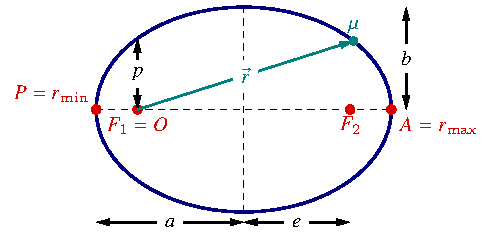
\includegraphics[width=0.5\textwidth]{pictures/central_force_ellipse.pdf}

	\caption{Quantities in an ellipse.}
	\label{fig:central_force_ellipse}
\end{figure}



First, we have $\epsilon$, which is called \Def{numerical eccentricity}:
\begin{center}
	$\epsilon < 1$: ellipse
	\qquad
	$\epsilon = 1$: parabola
	\qquad
	$\epsilon > 1$: hyperbola
\end{center}
Note that $\epsilon = 0$ represents a special form of ellipse, a circle. In terms of physical quantities,
\begin{equation}
	\eqbox{
		\epsilon = \sqrt{1 + 2 \frac{E L^2}{m k^2}}
	} \, .
\end{equation}
Since all quantities in the square root are greater than zero, except for the energy, statements about the form of the orbit can be translated to statements in terms of energy: $E < 0$ means $\epsilon < 1$ and thus an elliptical orbit, which matches our understanding of a bound orbit; $E >= 0$ then corresponds to unbound orbits like parabola or hyperbola.


$p$ is another prominent one, the \Def{semi-latus rectum} of the conic section, which basically determines the size of the orbit. It involves the same physical quantities as $E$ (but combined in a different way, it plays a different role than $\epsilon$) and reads
\begin{equation}
	\eqbox{
		p = \frac{L^2}{m k}
	}
	\, .
\end{equation}


These quantities play a sort of hybrid role because they can be interpreted physically or mathematically, via their role in the general description of conic sections (cf.~Fig.~\ref{fig:central_force_ellipse}). 


The lengths along these axes are called \Def[major axis]{major} and \Def{minor axis}, describing the longer and shorter axis. In Fig.~\ref{fig:central_force_ellipse}, we elect to draw the \Def{semi-major axis}
\begin{equation}
	\eqbox{
		a = \frac{p}{1 - \epsilon^2} = \frac{r_\mathrm{min} + r_\mathrm{max}}{2}
	}
\end{equation}
and \Def{semi-minor axis}
\begin{equation}
	\eqbox{
		b = \frac{p}{\sqrt{1 - \epsilon^2}} = \sqrt{r_\mathrm{min} r_\mathrm{max}}
	} \, ,
\end{equation}
as is commonly done (\enquote{semi} = half). Here we have chosen to also express them in terms of the minimal and maximal distance. In celestial mechanics, one calls those \Def{perihelion}\footnote{\enquote{Peri} $\hat{=}$ close, to memorize which point represents minimum/maximum.}
\begin{equation}
	\eqbox{
		r_\mathrm{min} = \frac{p}{1 + \epsilon}
	}
\end{equation}
and \Def{aphelion}
\begin{equation}
	\eqbox{
		r_\mathrm{max} = \frac{p}{1 - \epsilon}
	}
	\, .
\end{equation}
For the convention on the angle $\phi$ that we have chosen, these occur at $\phi = 0\degree, 180\degree$, respectively (where $\cos(\phi) = \pm 1$).

Besides the arithmetic ($a$) and geometric ($b$) mean of perihelion and aphelion, their harmonic mean also plays an important role. In fact, we have seen it already in the semi-latus rectum
\begin{equation}
	\eqbox{
		p = \qty(\frac{r_\mathrm{min}^{-1} + r_\mathrm{max}^{-1}}{2})^{-1} = \frac{b^2}{a}
	}
\end{equation}
which is the radius at $\phi = 90\degree, 270\degree$. Additionally, the numerical eccentricity receives a nicer interpretation: it is the coefficient of variation between perihelion, aphelion, i.e.
\begin{equation}
	\eqbox{
		\epsilon = \frac{r_\mathrm{max} - r_\mathrm{min}}{r_\mathrm{max} + r_\mathrm{min}}
	}
	\, .
\end{equation}
For completeness, we note that there is also another notion of eccentricity in the \Def{linear eccentricity}
\begin{equation}
	\eqbox{
		e = \epsilon a
	}
	\, .
\end{equation}\\

% -> nice expressions here: \url{https://en.wikipedia.org/wiki/Kepler%27s_laws_of_planetary_motion#First_law}


-> possibly some nice things on trajectory: \url{https://en.wikipedia.org/wiki/Kepler_orbit#Properties_of_trajectory_equation}



Let us get back to physics now. The first result of note is that, when fixing the position of body $2$, body $1$ performs an elliptical motion around it with the first body sitting at a focal point of this ellipse. (This is a direct consequence of the result we have calculated in Eq.~\eqref{eq:central_force_r_of_phi}, which shows that the reduced mass $\mu$ performs such a motion around the origin; body $1$ need not be in the origin for this interpretation to be true.) However, this is not how the actual orbit of body $1$ looks like, when viewed from a proper, inertial frame; similarly, in such a frame, body $2$ is not necessarily at rest for all times.

To obtain the trajectories of both bodies, we must use the transformations from $\vec{R}, \vec{r}$ back to $\vec{r}_{1, 2}$ in Eq.~\eqref{eq:trafo_com_components}. Those tranformation equations immediatelly tell us that, generally speaking, the physical trajectories of both bodies are ellipses (of different extent, determined by $\frac{\mu}{m_i} = \frac{m_j}{M} (1 - \delta_{ij})$ for the $i$-th body), and that they both have $\vec{R}$ in one of their focal points (as this is the constant offset from the focal point $O = (0, 0)$ of $\vec{r}$). We show some examples for different mass ratios $\flatfrac{m_1}{m_2}$ in Fig.~\ref{fig:central_force_orbits}.



% -> in the more physical/intuitive terms, this means m2 orbits around m1 in elliptical orbit, with m1 sitting at focal point (but note that these are all \emph{not} statements from an inertial frame, unless in Keplerian limit; normally, we have to transform to an inertial frame, which can be done by calculating $\vec{r}_1 = \vec{R} + \frac{m_2}{M} \vec{r}$; then we see that, in general, both bodies perform elliptical motion, and that they both have center of mass in focal point)

% -> fact that solution of problem using COM \enquote{looks like} problem for particle of mass $\mu$ only helps us make easy transition in Keplerian case, whence it allows direct transition from $\mu$ to $m_2 \approx \mu$; in most general case, it is probably not suited well because it can easily mess up intuition (about where center of mass is, whether in focal point or not, or how orbits of the two bodies look like); in this general setting, going to COM is really just a coordinate transformation applied to get easier solutions to the equations of motion, but for the really interesting, physical results we still have to map back to the initial (inertial) frame (though some limited statements can be inferred from $\vec{r}$ already, namely about motion of m2 around m1; ultimately, this is not relevant though, since actual motion of m2 might be substantially different)



\begin{figure}
	\centering

	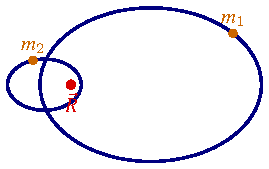
\includegraphics[height=0.1\textheight]{pictures/central_force_orbits.pdf}

	\caption{Some orbits. Keplerian limit is uppermost one \todo{fix plot}}
	\label{fig:central_force_orbits}
\end{figure}




		\subsection{Kepler's Laws}
From a historical point of view, the solution of the two-body problem in the way presented here was found by Newton, a few decades after Johannes Kepler famously formulated his three laws about the orbits of planets in our solar system. For Kepler, these laws were empirical insights gained from data collected by Tycho Brahe; for us, they will come quite naturally as corollaries from the general two-body and central-force problem over the last few subsections. To see that, let us consider the case $m_2 \gg m_1$, which means $M \approx m_2, \mu \approx m_1$.


Kepler considered two objects that interact gravitationally, which means the potential is given by
\begin{equation}
	\eqbox{
		V(r) = - \frac{G M m}{r}
	}
	\, .
\end{equation}
Here we have started to use $M$ for the mass $m_2$ of the larger body (the sun) and $m$ for the mass $m_1$ of the smaller body (the planet in consideration).




% mention fatal misconception by Kepler, trying to describe everything using ellipses? Which made things unbelievably complicated -> would have to read up on this, but sounds like a kind of funny anecdote



			\paragraph{First Law}

\begin{center}
	% The orbit of the relative coordinate $\vec{r}$ around the COM $\vec{R}$ is an ellipse with $\vec{R}$ at one of its foci. -> this is WRONG! Relative coordinate is not starting in COM, and COM is not always in focal point
	The orbit of every planet is an ellipse with the sun at one of the two foci.
\end{center}

% -> we are not satisfied with this, let's solve for the actual orbits (this part was done by Newton, a few decades after Kepler noted nature of orbits)


Other than the implication that all planets have inclination $< 1$, this is really just a corollary of planets orbiting the sun being an example of the two-body problem in a central force. Schematically, Fig.~\ref{fig:kepler_orbits} shows how the orbits of several planets look like; notice in particular how the sun is always in a focal point. In the Keplerian limit, Fig.~\ref{fig:central_force_ellipse} depicts accurately the orbit of a planet if we place $\vec{R}$ in $F_1$ (which is the origin in this plot, though this is not required), since $\vec{r}_1 \approx \vec{R}$ and $\vec{r}_2 \approx \vec{r}$.



\begin{figure}
	\centering

	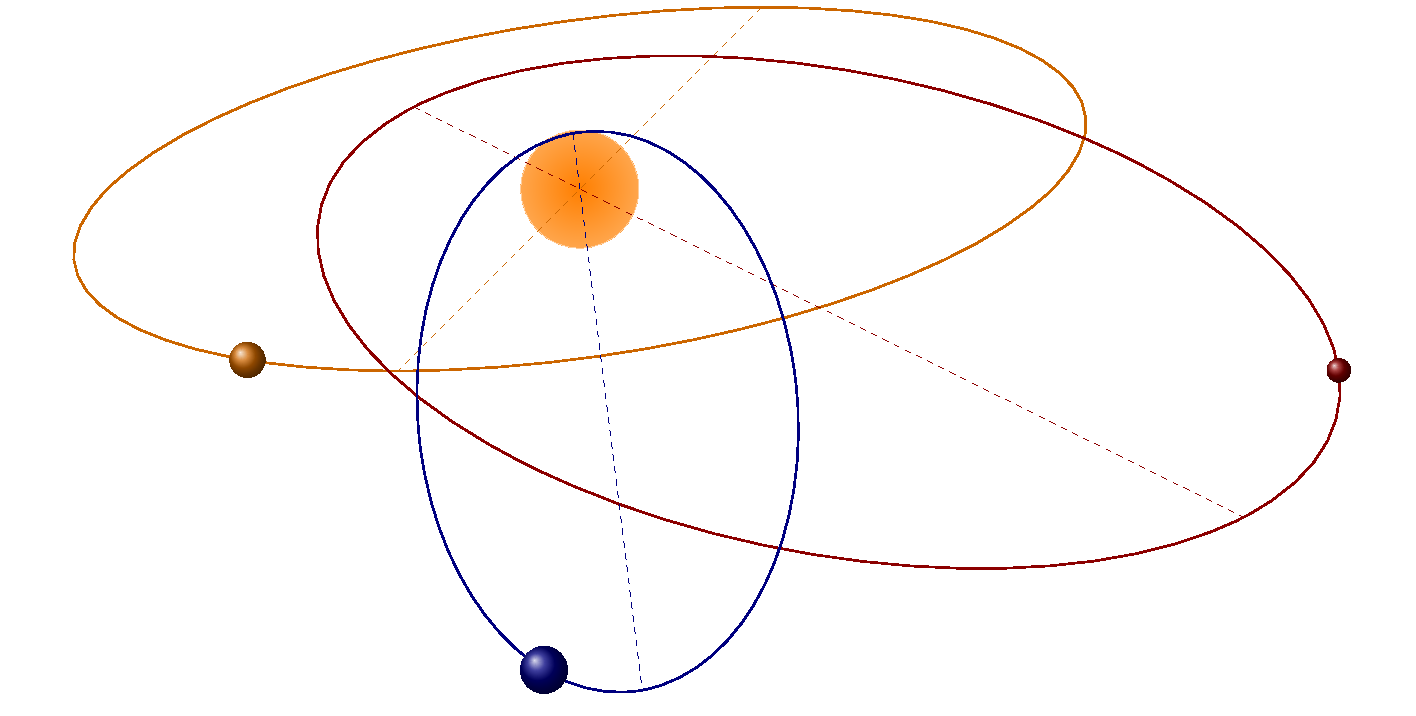
\includegraphics[width=0.5\textwidth]{pictures/central_force_planets.pdf}

	\caption{Some planet orbits. 3D, unlike in previous plots}
	\label{fig:kepler_orbits}
\end{figure}




			\paragraph{Second Law}
The first Keplerian law tells us the motion of a body in a central potential follows an elliptical orbit. In other words, the body moves in a plane. The second law can be stated as:

\begin{center}
	% A line segement connecting the two bodies sweeps out equal ares during equal time intervals.
	A line segement along the relative coordinate $\vec{r}$ sweeps out equal areas during equal time intervals.
\end{center}
\todo{really with center?}


In a more explicit (and perhaps modern) interpretation, the second law is usually stated in terms of angular momentum. We had seen that $\vec{L}$ is conserved, i.e.~constant in time (both direction and magnitude). The area swept out for a given time can be calculated as
\begin{equation}
	\eqbox{
		A = \int_{t_1}^{t_2} \frac{L}{2m} \, dt = \frac{L}{2m} (t_2 - t_1)
	} \, .
\end{equation}
This means we are already done proving Kepler's second law: the area swept out is a constant multiplied with the time interval. Due to its close relation to angular momentum, the second Keplerian law is often seen as an early formulation of conservation of angular momentum.

% -> notice how potential only depends on distance, not direction, crucial assumption here; moreover, this particular form of gradient means we have radial or quadratic force -> hmm nah, is general law, right? We only use chain rule here

% further characterization of the motion: for any force $\propto \vec{r}$, $\dot{\vec{L}} = \vec{r} \cross \vec{F} \propto \vec{r} \cross \vec{r} = 0$; in terms of potential, that means $\propto \frac{1}{r}$ or $\propto r^2$; so for central force problem as special case of this, we have angular momentum conservation


-> constancy of $L$ tells us same about velocity: for smaller $r$, we need larger $v$ to keep $L$ constant (which neglects dependence on angle between $\vec{r}, \vec{v}$, but point stands, think about periastron and apostron for example)


-> in Keplerian case, $\vec{R}$ coincides with $\vec{r}_1$; thus $\vec{L} = \vec{L}_{\vec{r}}$ and all claims involving angular momentum do not require so much case \todo{mention here or after starting Kepler section?}




			\paragraph{Third Law}
There exists a general formula for the area of an ellipse,
\begin{equation}
	A = \pi a b
	\, .
\end{equation}
However, we can also calculate the area in terms of other physical quantities by integrating Kepler's second law over an entire orbit. This results in
\begin{equation}
	A = T \frac{L}{2m}
\end{equation}
which in turn yields
\begin{equation}
	\eqbox{
		\frac{T^2}{a^3} = \frac{\pi^2 \mu k^2}{- 2 E^3} \frac{- 8 E^3}{k^3} = \frac{4\pi^2 \mu}{k}
	}
	\, .
\end{equation}
In other words, if we take two different bodies in a central force,
\begin{equation}
	\eqbox{
		\qty(\frac{T_1}{T_2})^2 = \qty(\frac{a_1}{a_2})^3
	} \, .
\end{equation}
For our solar system, this means the orbits of planets farther out in the solar system (larger $a$) have a longer orbital period $T$.



		\subsection{Collisions}
\todo{wouldn't that fit really well here?}



		\subsection{Scattering}
We have looked at $\epsilon < 1$ case extensively now, but what about $\epsilon \geq 1$. Formally, this is the case of hyperbolic trajectories and we can think of it as \enquote{collisions at a distance}: $m_1$ flies in, interacts with the potential generated by $m_2$, and flies off again. This is what physicists call \Def{scattering}. It occurs in a variety of places throughout virtually all physical theories (celestial bodies, nuclear physics, particles moving through the atmosphere, ...). % This is also the scope that we discuss it in, i.e.~we drop the assumption of gravitational interaction for now and return to a general central force. \todo{really? Even at this stage? Right now we just need conservative, don't we? -> hmm not 100\% sure, I think we assume central force actually}

% -> this is hyperbolic case, and there are some interesting dynamics going on as well; make transition to scattering, talk about deflection angle

% -> this central force problem not only occurs for celestial objects that pass by a planet or something, but all over the place in physics; another example is Rayleigh scattering of particles in the atmosphere (then talk about cross section)

We follow the discussion provided in \cite{Thornton_2003}, so we have to pay a little attention to the scope of certain formulas. 


We will analyze the situation from a frame (\enquote{lab frame}) where $m_2$ is initially at rest, while $m_1$ enters the frame with velocity $v_1$. Given this information (or equivalent one, like the charges if a Coulomb force is considered), the strength of the interaction taking place is entirely determined by $b$, the \Def{impact parameter}, which is the minimal distance of the particles if no force was acting (Fig.~\ref{fig:scattering}). $b$ determines what trajectories after scattering process look like, which can be encapsulated in the \Def{scattering angle} $\theta$.


The previous paragraph needs some clarification. It follows an argument from \cite{Thornton_2003}, which goes as follows: $b$ is sufficient to determine trajectories etc.~because all expression we saw for central force involved just energy $E$, potential $V$, angular momentum $L$. However, assuming that $m_2$ is at rest before the particles interact, the total angular momentum is given entirely by the angular momentum of $m_1$. Since we are free to choose a reference point for $\vec{L}$, we can choose to look at angular momentum of $m_1$ about $m_2$. For $m_1$ far away from $m_2$, this is given by
\begin{equation}
	L = m_1 v_1 b = b \sqrt{2 m_1 T'_1}
\end{equation}
where $v_1$ also refers to the velocity far away from $m_2$ (which just means the force exerted by $m_2$ has a negligible effect). Since the magnitude $L$ is conserved in a central force, $b$ is the quantity that determines the whole interaction (because mass, initial velocity are considered to be known).\footnote{It might be possible to get away with the less restrictive requirement of conserved angular momentum, not necessarily central force. But we chose to focus on central forces here.} The fact that we have to assume $\dot{L} = 0$ for this argument was not entirely obvious to me from reading the discussion in \cite{Thornton_2003}, which is why we emphasize it here.

-> also, $E = T'_1$ where $T'_1$ is kinetic energy far away from origin, since we have energy conservation (prime indicates we compute it in CMS)

% better justification of why $b$ is sufficient: ; we assume $E$ to be given (via mass, velocity) and $V$ as well (since nature of force is known); angular momentum of $m_1$ about $m_2$, however, can be expressed in terms of $b$ as $L = m_1 v_1 b$ (which is value of $L$ at particular point, but the magnitude of this value is conserved, so we can just use it); therefore, $b$ already determines quantities such as $r(\phi)$



\begin{figure}
	\centering

	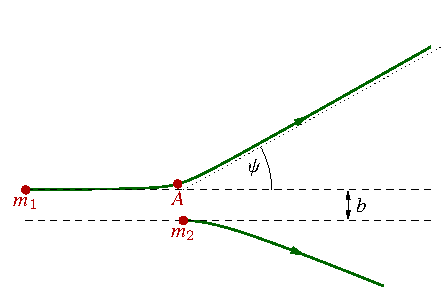
\includegraphics[width=0.5\textwidth]{pictures/scattering.pdf}

	\caption{Scattering. $\theta$ is same angle as $\psi$, but when viewed from CMS (whence motion of $m_1$ in this plot becomes motion of $\mu$; i.e.~$\theta$ is angle of trajectory of $m_1$ relative to $m_2$).}
	\label{fig:scattering}
\end{figure}



Treating the problem of scattering in a manner suitable for general application requires a paradigm shift because most of the time when we try to model scattering, we do not know what value $b$ exactly has. For planets as macroscopic objects, we may be able to find it; but when scattering electrons off of atoms, the story is very different because we have no way to measure $b$ in this case and thus no way to determine $\theta(b)$ exactly. Instead, we have to resort to assigning probabilities to ranges of values for $\theta$.

% -> i.e.~we would like to have $d\theta(db)$ for some range of $b$-values; factor of proportionality involves cross section

But first, we need some meaningful notions to describe the whole situation. For this, we can drop the assumption of a central force or conserved angular momentum, at least temporarily. Say we have particle beam with intensity $I$ that is incident on $m_2$. Then one can write the number of particles $dN$ scattered into a solid angle element $d\Omega'$ at scattering angle $\theta$ (and per unit time) as\footnote{The fact that we use $\theta$ means this is a definition in the CMS. We do this to be consistent with the treatment in \cite{Thornton_2003}, but note that a definition in the lab frame takes the same form, upon replacing $\theta \mapsto \psi, d\Omega' \mapsto d\Omega$ (since $\sigma(\theta) d\Omega' = \sigma(\psi) d\Omega$; must be the case since the amount of scattering into a given path of the sphere is something that does not depend on coordinates, and this is what both expressions represent in CMS, lab frame, respectively; this is visualized nicely in Fig.9-20 of \cite{Thornton_2003}).}
\begin{equation}\label{eq:cross_section_cms}
	\eqbox{
		dN = I \sigma(\theta) \, d\Omega'
	}
	\quad \Leftrightarrow \quad
	\eqbox{
		\sigma(\theta) = \dv{\sigma}{\Omega'} = \frac{1}{I} \dv{N}{\Omega'}
	}
\end{equation}
for some factor of proportionality $\sigma$. This factor quantifies how effectively particles from the beam are scattered into a specific solid angle element $d\Omega'$ by computing the ratio of particles scattered into $d\Omega'$ ($\dv{N}{\Omega'}$) and the total number of incident particles (per unit area and time, which is quantified by $I$). This ratio is called \Def{differential scattering cross section}.

% where the \Def{differential scattering cross section} $\sigma(\theta)$ quantifies \enquote{the number of interactions per target particle that lead to scattering into $d\Omega'$ at the angle $\theta$ (this is $dN$), divided by number of incident particles per unit area (this is $I$)}

% -> idea: intensity is also something like number per area (and time), but for the incoming particle stream; cross section thus compares incoming particles per area to particles per are (solid angle element) at a given angle; in other words, it tells us how effectively beam is scattered into the specific part of the sky that this solid angle element represents -> is number of particles scattered into specific solid angle element, normalized by total number of particles that are interacting (right?) -> intensity is power per area = energy per time and per area (= flux density)


The definition of $\sigma$ we have just provided can be used no matter what the nature of the force exerted by the second body is. For more detailed discussions, however, we now return to the assumption of a central force. This is a force that has axial symmetry, so
\begin{equation}
	d\Omega' = \sin(\theta) d\theta d\phi = 2\pi \sin(\theta) d\theta
\end{equation}
($d\Omega'$ is intended for integration, and we have carried one out now). We had stated that $b$ is sufficient to describe the scattering process, which means our goal is to find an expression for some range of scattering values in terms of a range of impact parameter values, i.e.~$d\theta = d\theta(db)$. For ease of analysis, we continue in the CMS and deal with the transformation back to the lab frame later on. In our axially symmetric setup, if we consider a disk of width $db$ and radius $b$ (centered on $b = 0$), then the area of this disk is just $2\pi b \, db$. Axial symmetry also implies all particles incident on this area are scattered to the same solid angle element $d\Omega'(\theta)$ (remember that we have \enquote{integrated out} the azimuthal dependence, the integration over the whole circumference of the circle here accounts for that), and since $\mathrm{number} = \mathrm{intensity} \cdot \mathrm{area}$,
% In our current setup, we have an intensity $I$ that is incident on the range $db$. Continuing continued axially symmetric must, upon multiplication with circumference $2\pi b$ (due to symmetry), correspond to particles scattered into $d\Omega'(\theta)$, i.e.
\begin{equation}
	\eqbox{
		I 2\pi b \, db = dN = - I \sigma(\theta) d\Omega' %= - I \sigma(\theta) 2\pi \sin(\theta) d\theta
	} \, .
\end{equation}
The minus comes from the fact that increasing the impact parameter $b$ decreases the amount of angular deflection $\theta$, i.e.~$\dv{b}{\theta} < 0$. Therefore, remembering the axial symmetry in expressing $d\Omega'$, we get
\begin{equation}\label{eq:cross_section_cms_2}
	\eqbox{
		\sigma(\theta) = \frac{b}{\sin(\theta)} \abs{\dv{b}{\theta}}
	} \, .
\end{equation}

This expression is helpful because for a central force interaction, one can show that the change in angle between the points of closest and largest distance is
\begin{equation}
	\Theta = \frac{\pi - \theta}{2} = \int_{r_\mathrm{min}}^{r_\mathrm{max}} \frac{L}{r^2 \sqrt{2 \mu \qty(E - V - \frac{L^2}{2 \mu r^2})}} \, dr
	\, .
\end{equation}
Using that $L = \mu v_1 b = b \sqrt{2 m_1 T'_1}$ (where, again, $T'_1$ denotes the kinetic energy \emph{before} any interaction with the central potential exerted from the origin takes place, and measured in the CMS), we obtain
\begin{equation}\label{eq:angle_as_func_of_b}
	\Theta = \int_{r_\mathrm{min}}^{\infty} \frac{b}{\sqrt{1 - \frac{b^2}{r^2} - \frac{U}{T'_1}}} \, dr
	\, .
\end{equation}
This determines how $\theta$ depends on $b$, which in turn allows determining $\sigma$ via Eq.~\eqref{eq:cross_section_cms_2}.\\


Having found an expression for the cross section in the CMS, our next task is to transform this expression to the lab frame. This involves a substantial amount of math (the calculation is based on $\sigma(\theta) d\Omega' = \sigma(\psi) d\Omega$), and the result also reflects this:
\begin{equation}\label{eq:cross_section_general}
	\eqbox{
		\sigma(\psi) = \eval{\sigma(\theta)}_{\theta = \arcsin(q \sin(\psi)) + \psi} \frac{\qty(1 \cos(\psi) + \sqrt{1 - q^2\sin[2](\psi)})^2}{\sqrt{1 - q^2\sin[2](\psi)}}
		, \quad q = \frac{m_1}{m_2}
	}
	\, .
\end{equation}
% -> note that this assumes $q \leq 1$; is fine, because we can always transform so that it is larger of the masses that is at rest, and reassign larger mass to $m_2$ -> uuum nope, we do not have something greater 1 in arcsin
Evaluating this expression is complicated for general $q$, but at least we have simple special cases: for $q = 1 \Leftrightarrow m_1 = m_2$, both particles get scattered at same angle in lab frame, so the relative angle between particles (which is what we have from CMS) being $\theta$, implies $\psi = \frac{\theta}{2}$, so that
\begin{equation}\label{eq:cross_section_q1}
	\eqbox{
		\sigma(\psi) = \eval{\sigma(\theta)}_{\theta = 2\psi} 4 \cos(\psi)
	}
\end{equation}
Similarly, for $m_1 \ll m_2 \Leftrightarrow q \approx 0$, the second particle remains at rest so that $\psi \approx \theta$ and
\begin{equation}\label{eq:cross_section_q0}
	\eqbox{
		\sigma(\psi) = \eval{\sigma(\theta)}_{\theta = \psi}
	}
\end{equation}



Although we have mostly used the symbol $\sigma$ for now, the cross sections used up until this point have been differential ones, i.e.~they only referred to an infinitesimal solid angle element. To obtain a \Def{total scattering cross section}, we thus have to integrate over the angular dependence
\begin{equation}
	\eqbox{
		\sigma = \int \sigma(\theta) \, d\Omega' = \int \sigma(\psi) \, d\Omega
	}
	\, .
\end{equation}

-> comment on different integration ranges

-> interpretation: this is what we should look at if we are interested in probability that any interaction with second particle $m_2$ takes place; resulting $\sigma$ is effective area of target particle (strongly interacting = large effective area)


\todo{show example? For solid sphere for example}




			\paragraph{Rutherford Scattering}
Let us discuss a particular example of a central force, namely once again
\begin{equation*}
	V(r) = - \frac{k}{r} \, ,
\end{equation*}
which describes, e.g., a massive particle in a gravitational field or a charged particle in a Coulomb field. For this force, one can evaluate Eq.~\eqref{eq:angle_as_func_of_b} to obtain
\begin{equation}
	\cos(\Theta) = \frac{k}{2 T'_1 \sqrt{1 + \qty(\frac{k}{2 T'_1})^2}}
\end{equation}
and this can be rearranged to
\begin{equation}
	\eqbox{
		b = \frac{k \cot(\theta/2)}{2 T'_1} = \frac{\mu k \cot(\theta/2)}{p^2}
	}
	\,. 
\end{equation}
Differentiating with respect to $\theta$ gives
\begin{equation}
	\dv{b}{\theta} = - \frac{k}{4 T'_1} \frac{1}{\sin[2](\theta/2)}
\end{equation}
and substitution of this into Eq.~\eqref{eq:cross_section_cms_2} then yields the final result
\begin{equation}\label{eq:rutherford_scat}
	\eqbox{
		\sigma(\theta) = \frac{k^2}{(4 T'_1)^2} \frac{1}{\sin[4](\theta/2)}
	}
	\, .
\end{equation}
This is the \Def{Rutherford scattering formula}. We see a strong dependence on $\theta$. Recall that $\sin[4](\theta/2) \simeq (\theta/2)^4$ for small angles, so the cross section falls off extremely steeply. On the other hand, there is no dependence on sign of $k$. That means we get same cross sections for attractive and repulsive forces.

Also, as a little aside, this classical result actually agrees with experimental evidence -- which means it agrees with QM-prediction of the same phenomenon (quite remarkably).\\


-> interesting: total cross section diverges!


For $m_1 = m_2$, $T'_1 = T_1/2$, so Eq.~\eqref{eq:rutherford_scat} becomes
\begin{equation}
	\sigma(\theta) = \frac{k^2}{(4 T_1)^2} \frac{1}{\sin[4](\theta/2)}
\end{equation}



    \section{Rigid Bodies}

now we go away from point particle/test mass


center of mass -> or introduce this in separate section on multi-particle systems?



first of all, there is no truly rigid body; relativity says maximum speed at which information can be transmitted is $c$, i.e.~finite, so if I push one end of a rod, the other one does not move immediately




given mass density $\rho(\vec{x})$ of a continuous body occupying some volume $V$, we can define its (total) mass
\begin{equation}
	M = \int_V dm
	% = \int_V \rho dV
	= \int_V \rho(\vec{x}) d^3x
\end{equation}
its center of mass
\begin{equation}
	\vec{X} = \frac{1}{M} \int_V \rho(\vec{x}) \vec{x} d^3x
\end{equation}
and its momentum
\begin{equation}
	\vec{P} = \int_V \rho(\vec{x}) \dot{\vec{x}} d^3x
\end{equation}

\todo{shouldn't we also have analogous expression for inner angular momentum? Or does this not exist for a rigid body?}

-> good for us that all of these are additive quantities (sometimes this is also called extensive, a notion coming from thermodynamics)


inner forces in a rigid body? Must be zero, because of the third law. Therefore, second law for rigid body reads
\begin{equation}
	\eqbox{
		\vec{F}_\mathrm{ext} = \dv{\vec{P}}{t}
	}
\end{equation}


its moment of inertia when rotated about some axis $\vec{n} = \frac{\vec{\omega}}{\omega}$
\begin{equation}
	I \coloneqq \vec{n}^T J \vec{n}, \quad J_{ij} = \int_V \rho(\vec{x}) \qty[\vec{x} \cdot \vec{x} \delta_{ij} - x_i x_j] d^3x
\end{equation}


component of $\vec{L} \parallel \vec{\omega}$:
\begin{equation}
	% \vec{L}_\omega = \vec{L} \cdot \vec{n} \underset{\todo{understand this}}{=} \vec{n}^T J \vec{n} \omega = \vec{M}_\mathrm{ext} \cdot \vec{n}
	\vec{L}_\omega = \vec{L} \cdot \vec{n} = I_\omega \vec{\omega} \cdot \vec{n} = \vec{n}^T J \vec{n} \omega \underset{\todo{understand this}}{=} \vec{M}_\mathrm{ext} \cdot \vec{n}
\end{equation}
hmm I mean we have $\vec{L} = I \vec{\omega}$ where $I$ is moment of inertia around $\vec{n}$

-> one has to exert moment of inertia around the axis of rotation in order to change the angular momentum (total angular momentum of the body)

-> not sure we can see this from the equation here; but this holds in general, right? Not just for rigid body




nice for work on rigid body: \url{https://en.wikipedia.org/wiki/Work_(physics)#Work_of_forces_acting_on_a_rigid_body}



gravitation of rigid bodies: \url{https://en.wikipedia.org/wiki/Shell_theorem}



		\subsection{Rotating Rigid Bodies}
talk about Euler angles



\end{document}